\documentclass[12pt]{article}\usepackage[]{graphicx}\usepackage[]{color}
%% maxwidth is the original width if it is less than linewidth
%% otherwise use linewidth (to make sure the graphics do not exceed the margin)
\makeatletter
\def\maxwidth{ %
	\ifdim\Gin@nat@width>\linewidth
	\linewidth
	\else
	\Gin@nat@width
	\fi
}
\makeatother

\definecolor{fgcolor}{rgb}{0.345, 0.345, 0.345}
\newcommand{\hlnum}[1]{\textcolor[rgb]{0.686,0.059,0.569}{#1}}%
\newcommand{\hlstr}[1]{\textcolor[rgb]{0.192,0.494,0.8}{#1}}%
\newcommand{\hlcom}[1]{\textcolor[rgb]{0.678,0.584,0.686}{\textit{#1}}}%
\newcommand{\hlopt}[1]{\textcolor[rgb]{0,0,0}{#1}}%
\newcommand{\hlstd}[1]{\textcolor[rgb]{0.345,0.345,0.345}{#1}}%
\newcommand{\hlkwa}[1]{\textcolor[rgb]{0.161,0.373,0.58}{\textbf{#1}}}%
\newcommand{\hlkwb}[1]{\textcolor[rgb]{0.69,0.353,0.396}{#1}}%
\newcommand{\hlkwc}[1]{\textcolor[rgb]{0.333,0.667,0.333}{#1}}%
\newcommand{\hlkwd}[1]{\textcolor[rgb]{0.7te37,0.353,0.396}{\textbf{#1}}}%

\usepackage{framed}
\makeatletter
\newenvironment{kframe}{%
	\def\at@end@of@kframe{}%
	\ifinner\ifhmode%
	\def\at@end@of@kframe{\end{minipage}}%
\begin{minipage}{\columnwidth}%
	\fi\fi%
	\def\FrameCommand##1{\hskip\@totalleftmargin \hskip-\fboxsep
		\colorbox{shadecolor}{##1}\hskip-\fboxsep
		% There is no \\@totalrightmargin, so:
		\hskip-\linewidth \hskip-\@totalleftmargin \hskip\columnwidth}%
	\MakeFramed {\advance\hsize-\width
		\@totalleftmargin\z@ \linewidth\hsize
		\@setminipage}}%
{\par\unskip\endMakeFramed%
	\at@end@of@kframe}
\makeatother

\definecolor{shadecolor}{rgb}{.97, .97, .97}
\definecolor{messagecolor}{rgb}{0, 0, 0}
\definecolor{warningcolor}{rgb}{1, 0, 1}
\definecolor{errorcolor}{rgb}{1, 0, 0}
\newenvironment{knitrout}{}{} % an empty environment to be redefined in TeX

\usepackage{alltt} % use larger type; default would be 10pt

\usepackage[T5]{fontenc}
\usepackage[utf8]{inputenc} % set input encoding (not needed with XeLaTeX)

%%% Examples of Article customizations
% These packages are optional, depending whether you want the features they provide.
% See the LaTeX Companion or other references for full information.

%%% PAGE DIMENSIONS
\usepackage{geometry} % to change the page dimensions
\geometry{letterpaper} % or letterpaper (US) or a5paper or....
\geometry{margin=1.2in} % for example, change the margins to 2 inches all round
% \geometry{landscape} % set up the page for landscape
%   read geometry.pdf for detailed page layout information

\usepackage{graphicx} % support the \includegraphics command and options

% \usepackage[parfill]{parskip} % Activate to begin paragraphs with an empty line rather than an indent

%%% PACKAGES
\usepackage{booktabs} % for much better looking tables
\usepackage{array} % for better arrays (eg matrices) in maths
\usepackage{paralist} % very flexible & customisable lists (eg. enumerate/itemize, etc.)
\usepackage{verbatim} % adds environment for commenting out blocks of text & for better verbatim
\usepackage{subcaption} % make it possible to include more than one captioned figure/table in a single float
\usepackage{float}
\usepackage{setspace}
\usepackage{pdflscape}
\usepackage{amsmath}
\usepackage{url}
\usepackage{multirow}
\usepackage{listings}
\usepackage{dcolumn}
%\usepackage[nolists]{endfloat}
\usepackage{bbm}
\usepackage{pdflscape}
\usepackage{pdfpages}

\usepackage{natbib}
\bibliographystyle{apsr}
\usepackage{hyperref}

\usepackage{tikz} 
\usetikzlibrary{arrows,decorations.pathmorphing,decorations.pathreplacing,backgrounds,fit,positioning,shapes.symbols,chains}

%%% HEADERS & FOOTERS
\usepackage{fancyhdr} % This should be set AFTER setting up the page geometry
\pagestyle{fancy} % options: empty , plain , fancy
\renewcommand{\headrulewidth}{0pt} % customise the layout...
\lhead{}\chead{}\rhead{}
\lfoot{}\cfoot{\thepage}\rfoot{}

%%% SECTION TITLE APPEARANCE
\usepackage{sectsty}
\allsectionsfont{\sffamily\mdseries\upshape} % (See the fntguide.pdf for font help)
% (This matches ConTeXt defaults)

%%% ToC (table of contents) APPEARANCE
\usepackage[nottoc,notlof,notlot]{tocbibind} % Put the bibliography in the ToC
\usepackage[titles,subfigure]{tocloft} % Alter the style of the Table of Contents
\renewcommand{\cftsecfont}{\rmfamily\mdseries\upshape}
\renewcommand{\cftsecpagefont}{\rmfamily\mdseries\upshape} % No bold!

%%% Some commands
\newcommand{\reg}{\texttt{regress} }
\newcommand{\1}{\mathbbm{1}}

\renewcommand\r{\right}
\renewcommand\l{\left}
\newcommand\E{\mathbbm{E}}
\newcommand\V{\mathbbm{V}}
\newcommand\Var{\mathbbm{V}}
\newcommand\avar{{\rm Avar}}
\newcommand\dist{\buildrel\rm d\over\sim}
\newcommand\iid{\stackrel{\rm i.i.d.}{\sim}}
\newcommand\ind{\stackrel{\rm indep.}{\sim}}
\newcommand\cov{{\rm Cov}}
\newcommand{\R}{\textbf{R} }
\newcommand{\Rcmd}[1]{{\large \texttt{#1}}}
\newcommand\indep{\protect\mathpalette{\protect\independenT}{\perp}}
\def\independenT#1#2{\mathrel{\rlap{$#1#2$}\mkern2mu{#1#2}}}
\DeclareMathOperator{\sgn}{sgn}
\DeclareMathOperator*{\argmin}{argmin}

\newcommand\Sum{\sum^N_{i=1}}
\newcommand\Prod{\prod^N_{i=1}}
\newcommand{\pderiv}[1]{\frac{\partial}{\partial #1}}
\newcommand{\B}[1]{\boldsymbol{#1}}
\newcommand{\logit}{\text{logit}}

%opening
\title{Vietnam's Tea Leaf Elections: \\
	Inferring Purpose for Authoritarian Elections from Post-election Responses to Local Defeats}
\author{Minh Trinh}

\begin{document}

\maketitle

\doublespacing

\section{Introduction}

An explanation for why authoritarian regimes choose to hold elections is that authoritarian elections may bring to dictators many benefits that outweigh the risk and cost of holding them. One particular benefit of authoritarian elections is information, which can be acquired by studying patterns of electoral returns across constituencies. The literature, however, has arrived at no consensus about what specific information authoritarian regimes seek to infer from elections. More critically, theories about information flow from authoritarian elections have failed to recognize that election results can be interpreted in multiple ways, among those some may be incompatible with or contradictory to others. How authoritarian leaders choose between competing interpretations of the same election result may shed light on their intention for holding elections. I focus in particular on the ``geographic distribution'' theory, which suggests that authoritarian leaders use elections to infer the geographic distribution of regime support in subnational units, and the ``local bureaucrats'' theory, which suggests that they use elections to monitor government officials in the same units, and seek to find out which theory applies in a situation when only one could hold true.

I analyze the responses by the Communist Party of Vietnam (CPV) to the defeats of candidates nominated by the central government (versus candidates nominated by local governments) in three legislative elections in 2007, 2011 and 2016 to identify which of these two theories describes better party's interpretation of election results and its motive for holding elections. I focus in particular on adjustments to central transfers from the central government to individual provinces. Because central transfers are wholly determined by the country's highest leadership, it is a good proxy to study the regime's decisions. I argue that the ``geographic distribution'' theory would predict that the CPV perceives defeats of central nominees as evidence of fledging popularity in specific provinces, and responds by increasing central transfers to these provinces in order to placate the public. On the other hand, the ``local bureaucrats'' theory would predict that it sees these defeats as signaling incompetence and/or disloyalty on the part of provincial bureaucrats who are in charge of managing elections, and thus decreases central transfers to the same provinces to punish these bureaucrats. Adjudicating between these two theories thus requires identifying the causal effect of election defeats on central transfers to provinces. To accomplish this goal, I employ linear fixed-effects regressions over an appropriate subset of the data to achieve identification, and rely on randomization inference to conduct finite-sample tests of the main hypotheses. Additional analyses using the synthetic control method provide robustness checks.

My analysis shows that the CPV generally responds to electoral upsets by increasing transfers to the provinces where defeats occurred. This pattern of response would be expected in a regime that uses elections to gather information on the geographic distribution of regime support. Through its empirical findings, this paper contributes to literature by demonstrating an approach to test competing theories of authoritarian elections. It also highlights the potential for discord between these theories, which could go unnoticed when theory-building advances too far ahead of theory-testing. The findings also suggest that authoritarian regimes may prefer to use elections as a tool for bottom-up rather than top-down accountability, in the sense that they rely on election results to appropriately respond to public dissatisfaction rather than to punish under-performing bureaucrats. Although this shows that authoritarian regimes are capable of meeting public dissatisfaction with concessions, it also echoes the literature's other findings that seemingly democratic institutions may end up reinforcing the durability of authoritarianism \citep[e.g.][]{BoixSvolik2013, GandhiPrzeworski2007}.

The paper begins in section \ref{sec:info} by reviewing the literature on the ``information flow'' theories of authoritarianism. As part of the review, the paper draws attention to the two potentially contradictory theories of ``geographic distribution'' and ``local bureaucrats.'' Then, in section \ref{sec:vietnam}, I provide information about the National Assembly election in Vietnam, and suggest how the Vietnam case could be used to test these two theories. Section \ref{sec:methods} then discusses my empirical approaches, and section \ref{sec:results} summarizes the results. Section \ref{sec:conclusion} reviews the results and their implications, then finally concludes.


\section{Authoritarian Elections as Information}
\label{sec:info}
A large portion of the literature on authoritarian elections has drawn attention to the benefits these elections may bring to authoritarian regimes, and suggested that such benefits can be large enough for elections to become a rational strategy for these regimes to pursue. Existing theories have portrayed elections as a platform for power-sharing, providing non-violent means for elites to contest over patronage \citep{LustOkar2006} or for dissidents to express dissatisfaction \citep{AR2005}. Elections are also said to help "divide and conquer" the opposition and co-opt some of them into the regime \citep{LustOkar2005}, or as a "show of strength" for the regime to impress upon its opponents the invulnerability of its rule and futility of resistance \citep{Geddes2005}. 

In addition to these explanations, a substantial literature on the ``information flow'' theories of authoritarian institutions\footnote{I owe this term, and the classification of theories of authoritarian institutions, to \cite{Hou2017}} has found that authoritarian regimes use nominally democratic institutions to gather information that would help them rule more efficiently. Elections and the results they generate serve this purpose particularly well. \cite{Geddes2005} for instance suggests that authoritarian regimes can look at election results to know how popular or strong their opposition is. In a similar but more sophisticated argument, \cite{Miller2015} finds that autocratic regimes use elections to estimate citizen dissatisfaction with the regime. The logic is that because autocratic regimes ensure that citizens face significant costs -- either in the form of punishment or withheld benefits -- when voting against the ruling party, voters would only dare to do so when they are genuinely dissatisfied. Negative election results, in particular electoral shocks, thus credibly communicate the true level of dissatisfaction, allowing the ruling regimes to alter its policy with an optimal level of responsiveness. An even more nuanced argument suggests that the variation in election results across constituencies shed light not on the general \textit{level}, but on the sub-national \textit{distribution} of regime support or dissatisfaction. Autocratic leaders can then use this information to identify opposition strongholds to suppress \citep{Magaloni2006, Blaydes2008} or marginal districts to buy off \citep{Reed2001, Magaloni2006}. Additionally, election results also convey information about the competence or loyalty of individuals within the regime machinery, in particular the government bureaucrats tasked with managing the elections and delivering results that the regime wants \citep{Magaloni2006, Blaydes2008}. Finally, unexpectedly strong performance by regime outsiders can also alert the regimes to potential threats, or indicate for them which elites should be co-opted into the regime \cite{LustOkar2005}.

\subsection{Local election defeats as high-information events}
It is possible to extend the ``information flow'' theories to argue that authoritarian elections are the most informative when they result in \textit{some} upsets for the regime. Under authoritarian regimes, electoral upsets are rarely expected but never impossible, even when the ruling regimes possess a ``menu of manipulation'' they can use to ensure favorable results \citep{Schedler2002Menu}. In particular, parliamentary elections under authoritarian regimes do sometimes lead to \textit{local defeats} -- defeats by regime candidates in local constituencies they run in. 

Local defeats are often a result of ambitious and innovative strategies by the opposition \citep{BunceWolchik2010} or certain regime weaknesses \citep{LevistkyWay2010}, but even in the case of dominant- or single-party regimes where competition is muffled \citep{Schedler2002} and the regime is strong \citep{BunceWolchik2010}, local defeats may still happen even if much less frequently. To begin with, authoritarian leaders may be aware that election fraud diminishes the informational value of elections \citep{Wintrobe2000}, and thus volunteer to refrain from excessive fraud on election day. Instead they may choose to tilt the playing field through pre-election manipulation of electoral institutions \citep{DiazMagaloni2001, Pepinsky2009, MaleskySchuler2011}, which reduces but does not eliminate the risk of losing for some of the regime's candidates. Additionally, competition under dominant- or single-party regimes also takes place more vigorously along unofficial cleavages like the center-periphery divide. Indeed, even when all the candidates compete under the same party banner, some of them may still represent local interests that run counter to that of the central party leadership. Such conflict of interest exists even in extremely institutionalized single-party regimes like China \citep{Manion2014} or Vietnam \citep{MaleskySchuler2011}. Victories by candidates representing the peripheral interests can be considered the dominant- or single-party regime's version of local defeats.
	
Since authoritarian regimes rarely suffer and thus do not expect such unsatisfactory results, any defeat would provide a data point so different from their informational prior that dictators can tell it contains more signal than noise. Indeed, whereas most variation in vote share can be attributed to random noise, only a true aberration could lead to a regime vote share low enough to produce a defeat. Thus, if a regime is truly using elections as an information gathering tool, it should always pay attention to any instance of local defeat, perhaps more than to vote share \textit{per se}. Depending on the regime's interpretation, a local defeat credibly signals either low regime popularity vis-\`{a}-vis the opposition, or unsatisfactory performance by regime agents on the ground.

\subsection{Multiple interpretations of local defeats}
While local defeats may truly represent high-information events, it is not straightforward how authoritarian leaders interpret such information. Most plausibly, dictators' interpretations for election results are guided by the original purpose they have for holding these elections -- they expect the very kind of information they intend to collect. Each ``information flow'' theory thus implies a different interpretation of election results, depending on which purpose that theory posits authoritarian elections serve.

But even as these theories lays out various ways authoritarian regimes \textit{may} interpret information from election defeats, it provides no guidance in determining in which of these ways they actually \textit{do} interpret this information. Existing works have only considered a small subset of theories at once, and have not conducted many comparative evaluation between pairs of theories to identify which theory fits better with empirical evidence. The one-country case studies that dominate this literature \citep{LustOkar2005, Geddes2005, Magaloni2006, Blaydes2008} often devote more effort proposing new theories rather than testing old ones. The result is an abundance of claims about what information authoritarian regimes seek from elections, but no clear conclusion about which claim carries the most weight. This gap in the literature is consequential because these theories are not always perfectly compatible, and thus cannot be all true. For understanding of authoritarian elections to advance, it is necessary to both explore more explicitly the conditions that make some theories more plausible than others, and subject these theories to more rigorous tests under these conditions.

\subsection{Interpretations of defeats imply post-election responses}

One way to test a claim about the informational value of authoritarian elections is to study changes in the dictators' behaviors in response to election results. Because every ``information flow'' theory rests on the premise that authoritarian leaders collect information from elections \textit{to calibrate their actions}, it is natural to expect that the large amount of information from local defeats will trigger a behavioral change. Furthermore, we only need to assume that authoritarian regimes prefer winning over losing to believe that they would do something to avoid future repetition of these defeats. 

In either case, a regime's post-election response should be informed by the information they have collected. More specifically, how the regime interprets the defeats will influence its thinking about who or what is responsible for the defeats, and consequently what actions should be done to whom to rectify the situation. Figure \ref{fig:Theory} lists for each prevalent theory of authoritarian elections the implied purpose for holding elections, the interpretation of election defeats that corresponds to each purpose, and then the post-election response that logically follows. Not every theory predicts a post-election response: according to the ``power-sharing'' theories, local defeats are expected and accepted by-products of elections, and should happen for the offer of power-sharing to be credible \citep{AR2005, Cox2009}. Other theories, such as the co-optation theory \citep{LustOkar2005}, predict post-election responses even if information is not the primary motive for elections. For the ``information flow'' theories, however, post-election responses are not directly predicted but should be expected as a necessary auxiliary outcome: what good is \textit{information} if it does not help \textit{inform} behaviors?

The leverage for testing theories of authoritarian elections come from the possibility that, within specific contexts, the logical post-election response to one interpretation of election results may be counterproductive to another interpretation and vice versa. When this happens, the two theories that predict these two interpretations are said to be outcome-incompatible (henceforth in this paper, I will use the terms ``incompatible'' and ``incompatibility'' in this sense). In this case, if an outcome is to be observed, it is only possible that the regime does not hold both interpretations, which necessarily follows that at least one theory is not applicable to the case. Not every pair of theories is prone to such incompatibility: the outcomes predicted by each of \cite{Miller2015} and \cite{Geddes2005}, for example, are very likely to apply to the other's theory. The next section, however, will focus on two theories that are especially likely to conflict.

\subsection{''Geographic distribution'' vs. ``local bureaucrats''}
Among the ``information flow'' theories, two are particularly at risk of diametrically contradicting each other, yet they are advanced in the same works without acknowledgment of potential conflicts. One theory suggests that election results provide information on the geographic distribution of support and dissent (henceforth the ``geographic distribution'' theory), whereas the other suggests that election results reveal individual local level party bureaucrats' level of competence or even level of loyalty to the central leadership (henceforth the ``local bureaucrats'' theory), and both of them are given equal spotlight in the two seminal works of \cite{Magaloni2006} and \cite{Blaydes2008}. 

Both scholars posit that electoral results provide information about the geographic distribution of support and dissent for the ruling regime. In Mexico, \cite{Magaloni2006} finds that areas where the ruling PRI captured a greater vote share were deemed as centers of government support, whereas areas with low PRI vote shares were considered opposition strongholds. Similarly, for Egypt, \cite{Blaydes2008} remarks that “election results provide the regime with a map of areas of political support for the opposition.” In both cases, the two authoritarian governments were able to know which sub-national units have higher or lower concentration of regime supporters by looking at where they received a higher or lower vote share. In Mexico, the PRI used this information to reward their supporters, whereas in Egypt the regime instituted a “punishment regime” in opposition strongholds by withholding their public goods investment.

In parallel, both \cite{Magaloni2006} and \cite{Blaydes2008} also suggest that election results provide information about the competence and loyalty of lower-level party members. In both countries, the task of mobilizing voters on behalf of the ruling party is delegated to lower-level party bureaucrats, with the national level playing little to no direct role. These bureaucrats are not candidates themselves, but play important role in making sure that the ruling party’s candidates get elected. Election results, reflected through turnout as well as through the ruling party' share of the votes, are then perceived as a function of how well these sub-national party members do their job. \cite{Blaydes2008} notes further that a failure to deliver good results may also be a symptom of disloyalty, for example when a local party member forgoes careerist goals within the ruling party to pursue short-term material gains offered by the local opposition candidates by mobilizing on behalf of the opposition instead.\footnote{In Mexico, \cite{Larreguy2016} show that the PRI also extends this method of evaluation to assess the vote-buying performance of local brokers.}

Although each of these two theories of authoritarian elections make sense on its own, neither \cite{Magaloni2006} nor \cite{Blaydes2008} acknowledge fully that they can be incompatible within one single case. From the perspective of the authoritarian leaders, the level of popular support in a province and the level of competence or loyalty of the party bureaucrats in the same province are two different narratives explaining a same outcome, at the same level of disaggregation. Thus, when explaining an electoral upset in a certain province, the first theory would suggest that regime leaders attribute the defeat to the lack of supporters in this province, but the second would suggest they attribute it to the bureaucrats managing the election there. It may be suggested that both theories hold true and the regime believes in both narratives, but even then it remains impossible for the regime to divide blame attribution for the defeat on these distinct causes without putting too much weight on one and too little on the other.\footnote{In statistical lingo, the ruling party is unable to point-identify how much each factor contributes to the bad result. To achieve point-identification it may be necessary to hold one factor constant or ignorable, for example by randomly assigning bureaucrats to provinces. Most readers would agree though that it is unreasonable to expect that politicians always see and behave like social scientists.} As we will see in the next section, the need to adjudicate between these two narratives becomes acute when they recommend entirely different policy responses to the same situation. In this case, the regime's ability to decide on the one policy to implement as part of a standard operating procedure rests upon its ability to pre-commit to one narrative to believe in.

\begin{figure}[H]

\centering
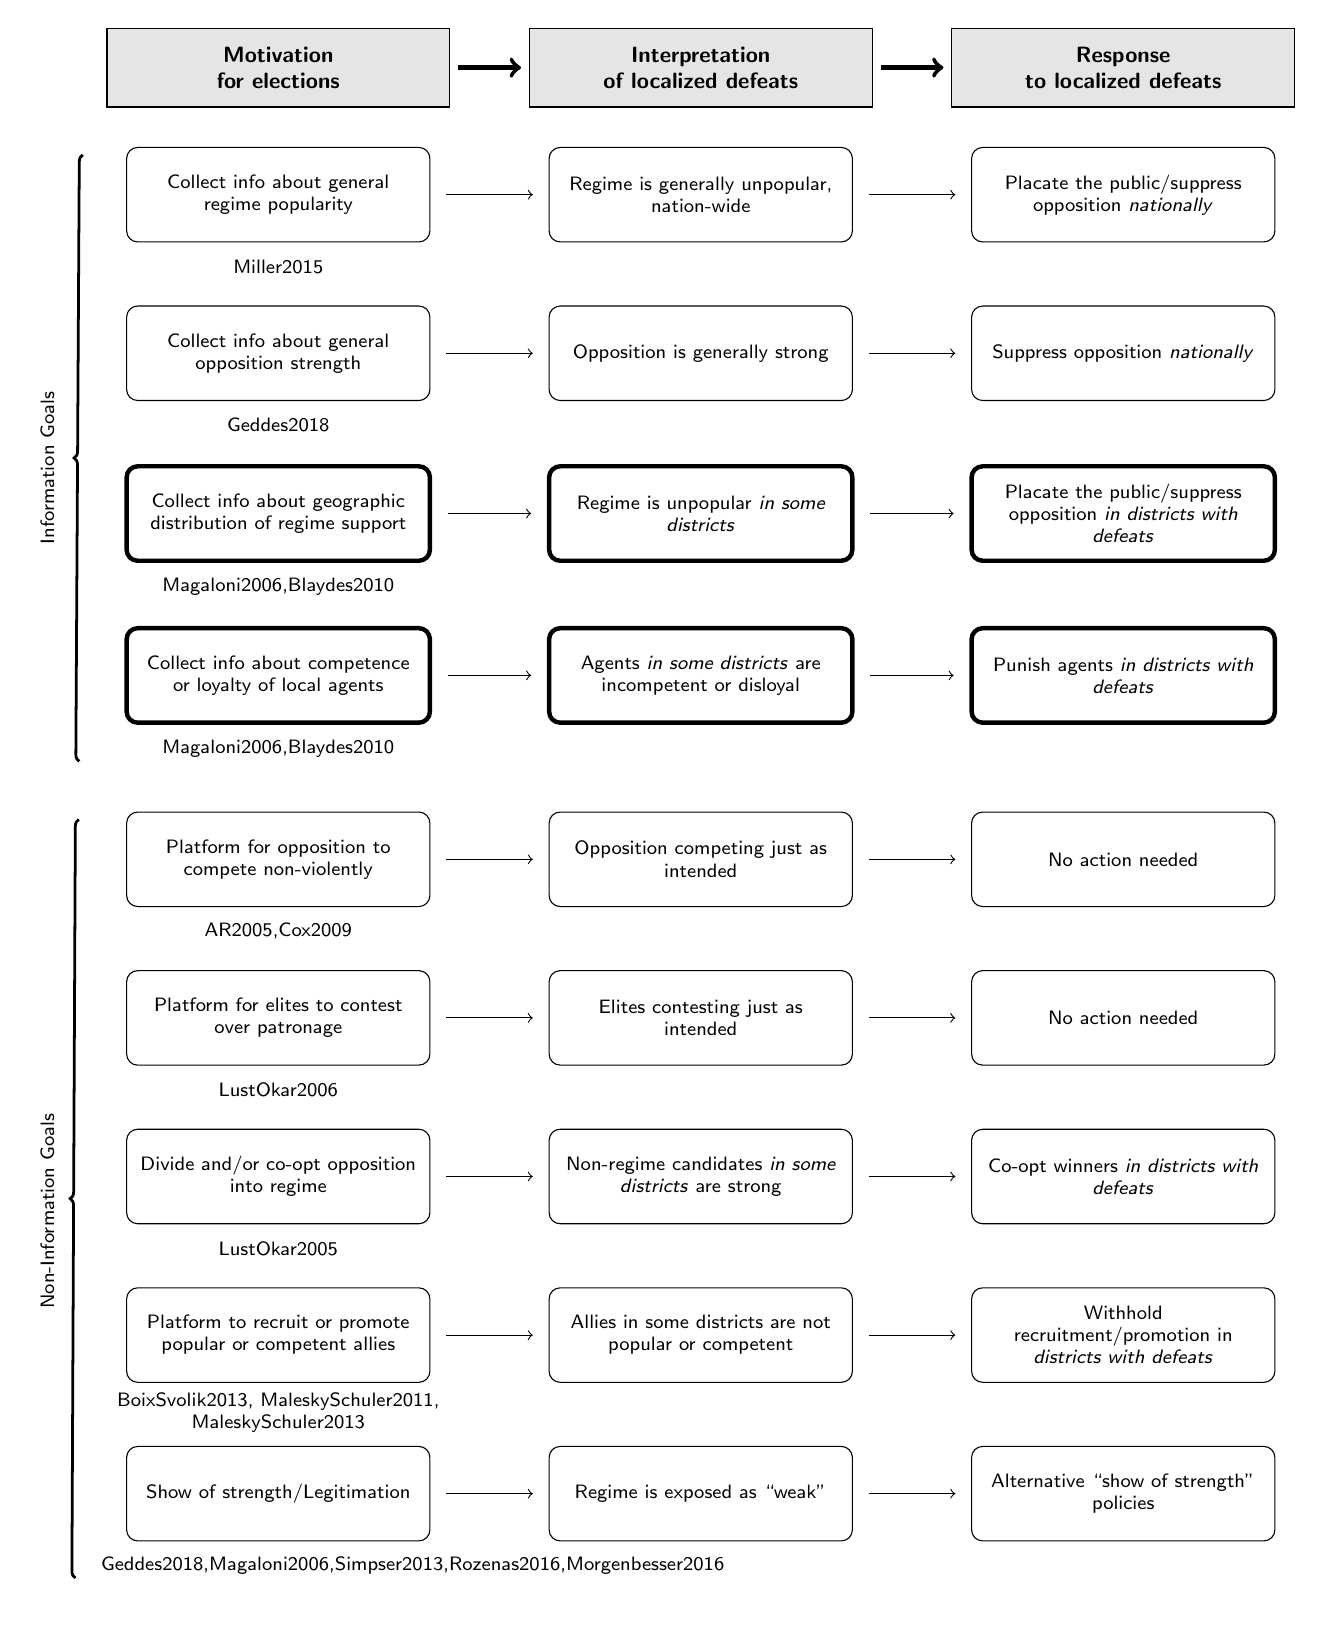
\begin{tikzpicture}
[node distance = 1cm, auto,font=\footnotesize,
% STYLES
every node/.style={node distance=3cm},
% The title style is used to draw the main title
title/.style={rectangle, draw, fill=black!10, inner sep=5pt, text width=4cm, text badly centered, minimum height=1cm, font=\bfseries\footnotesize\sffamily},
% The subtitle style is used to draw the title below main title
subtitle/.style={rectangle, inner sep= 2pt, minimum height=.5cm, node distance=0.25cm, text width=4.5cm, text badly centered, font=\scriptsize\sffamily},
% The theory style is used to draw nodes for each theory
theory/.style={rectangle, rounded corners, draw, minimum height=1.2cm, inner sep= 5pt, text width=3.5cm, node distance=0.25cm, text badly centered, font=\scriptsize\sffamily}]

%%%% Top nodes %%%%
\node [title] (interpretation) {Interpretation\\of localized defeats};
\node [title, left=1cm of interpretation] (intention) {Motivation\\for elections};
\node [title, right=1cm of interpretation] (response) {Response\\to localized defeats};

%% Top nodes subtitle

% Intention
%\node [subtitle, below=0.2cm of intention] (sub-intention) {for\\
%	authoritarian elections};

% Interpretation
%\node [subtitle, below=0.2cm of interpretation] (sub-interpretation) {of\\
%	localized defeats};

% Response
%\node [subtitle, below=0.2cm of response] (sub-response) {to\\
%	localized defeats};

%%%% Theory nodes %%%%
% B1
\node [theory, below=0.5cm of intention] (B1-intention) {Collect info about general regime popularity};
\node [subtitle, below=0.05cm of B1-intention] (B1-sub-intention) {\citep{Miller2015}};

\node [theory, below=0.5cm of interpretation] (B1-interpretation) {Regime is generally unpopular, nation-wide};
\node [subtitle, below=0.05cm of B1-interpretation] (B1-sub-interpretation) {};

\node [theory, below=0.5cm of response] (B1-response) {Placate the public/suppress opposition \textsl{nationally}};
\node [subtitle, below=0.05cm of B1-response] (B1-sub-response) {};

% B2
\node [theory, below=0.8cm of B1-intention] (B2-intention) {Collect info about general opposition strength};
\node [subtitle, below=0.05cm of B2-intention] (B2-sub-intention) {\citep{Geddes2018}};

\node [theory, below=0.8cm of B1-interpretation] (B2-interpretation) {Opposition is generally strong};
\node [subtitle, below=0.05cm of B2-interpretation] (B2-sub-interpretation) {};

\node [theory, below=0.8cm of B1-response] (B2-response) {Suppress opposition \textsl{nationally}};
\node [subtitle, below=0.05cm of B2-response] (B2-sub-response) {};

% B3
\node [theory, below=0.8cm of B2-intention, ultra thick] (B3-intention) {Collect info about geographic distribution of regime support};
\node [subtitle, below=0.05cm of B3-intention] (B3-sub-intention) {\citep{Magaloni2006,Blaydes2010}};

\node [theory, below=0.8cm of B2-interpretation, ultra thick] (B3-interpretation) {Regime is unpopular \textsl{in some districts}};
\node [subtitle, below=0.05cm of B3-interpretation] (B3-sub-interpretation) {};

\node [theory, below=0.8cm of B2-response, ultra thick] (B3-response) {Placate the public/suppress opposition \textsl{in districts with defeats}};
\node [subtitle, below=0.05cm of B3-response] (B3-sub-response) {};

% B4
\node [theory, below=0.8cm of B3-intention, ultra thick] (B4-intention) {Collect info about competence or loyalty of local agents};
\node [subtitle, below=0.05cm of B4-intention] (B4-sub-intention) {\citep{Magaloni2006,Blaydes2010}};

\node [theory, below=0.8cm of B3-interpretation, ultra thick] (B4-interpretation) {Agents \textsl{in some districts} are incompetent or disloyal};
\node [subtitle, below=0.05cm of B4-interpretation] (B4-sub-interpretation) {};

\node [theory, below=0.8cm of B3-response, ultra thick] (B4-response) {Punish agents \textsl{in districts with defeats}};
\node [subtitle, below=0.05cm of B4-response] (B4-sub-response) {};

% A1
\node [theory, below=1.1cm of B4-intention] (A1-intention) {Platform for opposition to compete non-violently};
\node [subtitle, below=0.05cm of A1-intention] (A1-sub-intention) {\citep{AR2005,Cox2009}};

\node [theory, below=1.1cm of B4-interpretation] (A1-interpretation) {Opposition competing just as intended};
\node [subtitle, below=0.05cm of A1-interpretation] (A1-sub-interpretation) {};

\node [theory, below=1.1cm of B4-response] (A1-response) {No action needed};
\node [subtitle, below=0.05cm of A1-response] (A1-sub-response) {};

% A2
\node [theory, below=0.8cm of A1-intention] (A2-intention) {Platform for elites to contest over patronage};
\node [subtitle, below=0.05cm of A2-intention] (A2-sub-intention) {\citep{LustOkar2006}};

\node [theory, below=0.8cm of A1-interpretation] (A2-interpretation) {Elites contesting just as intended};
\node [subtitle, below=0.05cm of A2-interpretation] (A2-sub-interpretation) {};

\node [theory, below=0.8cm of A1-response] (A2-response) {No action needed};
\node [subtitle, below=0.05cm of A2-response] (A2-sub-response) {};

% C1
\node [theory, below=0.8cm of A2-intention] (C1-intention) {Divide and/or co-opt opposition into regime};
\node [subtitle, below=0.05cm of C1-intention] (C1-sub-intention) {\citep{LustOkar2005}};

\node [theory, below=0.8cm of A2-interpretation] (C1-interpretation) {Non-regime candidates \textsl{in some districts} are strong};
\node [subtitle, below=0.05cm of C1-interpretation] (C1-sub-interpretation) {};

\node [theory, below=0.8cm of A2-response] (C1-response) {Co-opt winners \textsl{in districts with defeats}};
\node [subtitle, below=0.05cm of C1-response] (C1-sub-response) {};

% C2
\node [theory, below=0.8cm of C1-intention] (C2-intention) {Platform to recruit or promote popular or competent allies};
\node [subtitle, below=0.05cm of C2-intention] (C2-sub-intention) {\citep{BoixSvolik2013, MaleskySchuler2011, MaleskySchuler2013}};

\node [theory, below=0.8cm of C1-interpretation] (C2-interpretation) {Allies in some districts are not popular or competent};
\node [subtitle, below=0.05cm of C2-interpretation] (C2-sub-interpretation) {};

\node [theory, below=0.8cm of C1-response] (C2-response) {Withhold recruitment/promotion in \textit{districts with defeats}};
\node [subtitle, below=0.05cm of C2-response] (C2-sub-response) {};

% D1
\node [theory, below=0.8cm of C2-intention] (D1-intention) {Show of strength/Legitimation};
\node [subtitle, below=0.05cm of D1-intention] (D1-sub-intention) {\citep{Geddes2018,Magaloni2006,Simpser2013,Rozenas2016,Morgenbesser2016}};

\node [theory, below=0.8cm of C2-interpretation] (D1-interpretation) {Regime is exposed as ``weak''};
\node [subtitle, below=0.05cm of D1-interpretation] (D1-sub-interpretation) {};

\node [theory, below=0.8cm of C2-response] (D1-response) {Alternative ``show of strength'' policies};
\node [subtitle, below=0.05cm of D1-response] (D1-sub-response) {};

%%%% Side theory category nodes %%%%

% B
\node [subtitle, left=1cm of B1-intention.north west, rotate=90, text width = 8cm] (information) {Information Goals};

\draw [decorate,decoration=brace, line width=1pt] 
([xshift=-0.2cm, yshift=0.1cm]B4-sub-intention.south west) -- ([xshift=-0.55cm, yshift=-0.1cm]B1-intention.north west);

% A, C and D together
\node [subtitle, left=1cm of A1-intention.north west, rotate=90, text width = 10cm] (non-information) {Non-Information Goals};

\draw [decorate,decoration=brace, line width=1pt] 
([xshift=-0.25cm, yshift=0.1cm]D1-sub-intention.south west) -- ([xshift=-0.6cm, yshift=-0.1cm]A1-intention.north west);

%% A
%\node [subtitle, left=0.6cm of A1-intention.north west, rotate=90, text width = 4.4cm] (power-sharing) {``Platform''/``Power-sharing''};
%
%\draw [decorate,decoration=brace, line width=1pt] 
%([xshift=-0.2cm, yshift=0.1cm]A2-sub-intention.south west) -- ([xshift=-0.2cm, yshift=-0.1cm]A1-intention.north west);
%
%% C
%\node [subtitle, left=0.6cm of C1-intention.north west, rotate=90, text width = 1.9cm] (co-optation) {``Co-optation''};
%
%\draw [decorate,decoration=brace, line width=1pt] 
%([xshift=-0.2cm, yshift=0.1cm]C2-sub-intention.south west) -- ([xshift=-0.2cm, yshift=-0.1cm]C1-intention.north west);
%
%% D
%\node [subtitle, left=0.6cm of D1-intention.north west, rotate=90, text width = 2cm] (show-of-strength) {``Demonstration''};
%
%\draw [decorate,decoration=brace, line width=1pt] 
%([xshift=-0.2cm, yshift=0.1cm]D1-sub-intention.south west) -- ([xshift=-0.2cm, yshift=-0.1cm]D1-intention.north west);


%%%%%%%%%%%%%%%%

% Draw the links between forces
\path[->,ultra thick, shorten >=.1cm, shorten <=.1cm] 
(intention) edge (interpretation)
(interpretation) edge (response);

\path[->, shorten >=.2cm, shorten <=.2cm] 
(A1-intention) edge (A1-interpretation)
(A1-interpretation) edge (A1-response);

\path[->, shorten >=.2cm, shorten <=.2cm] 
(A2-intention) edge (A2-interpretation)
(A2-interpretation) edge (A2-response);

\path[->, shorten >=.2cm, shorten <=.2cm] 
(B1-intention) edge (B1-interpretation)
(B1-interpretation) edge (B1-response);

\path[->, shorten >=.2cm, shorten <=.2cm] 
(B2-intention) edge (B2-interpretation)
(B2-interpretation) edge (B2-response);

\path[->, shorten >=.2cm, shorten <=.2cm] 
(B3-intention) edge (B3-interpretation)
(B3-interpretation) edge (B3-response);

\path[->, shorten >=.2cm, shorten <=.2cm] 
(B4-intention) edge (B4-interpretation)
(B4-interpretation) edge (B4-response);

\path[->, shorten >=.2cm, shorten <=.2cm] 
(C1-intention) edge (C1-interpretation)
(C1-interpretation) edge (C1-response);

\path[->, shorten >=.2cm, shorten <=.2cm] 
(C2-intention) edge (C2-interpretation)
(C2-interpretation) edge (C2-response);

\path[->, shorten >=.2cm, shorten <=.2cm] 
(D1-intention) edge (D1-interpretation)
(D1-interpretation) edge (D1-response);


\end{tikzpicture} 
\caption{Key theories of authoritarian elections and their predictions about how regime leaders perceive and respond to localized defeats. Two theories most relevant to the Vietnam case are highlighted with bold borders.}
\label{fig:Theory}
\end{figure}


\section{Authoritarian Elections in Vietnam}
\label{sec:vietnam}
To test whether leaders in strong authoritarian regimes prefer to use elections to learn about the geographic distribution of regime support or about individual party bureaucrats, this paper will make use of Vietnam as a test case. Vietnam is a single-party state with a strong Communist party, and thus should be a representative case for most theories about institutionalized single-party states. In addition, the high level of control the Communist Party of Vietnam (CPV) has over elections \citep{MaleskySchuler2011} means that local defeats are rare, and that defeats that did happen are more likely to be signal than noise. Finally, in Vietnam the top leaders in its 63 provinces are outsiders appointed by the central leadership, but day-to-day government affairs at lower levels are conducted by officials who are often native to the locality they serve in.\footnote{The distinction between two types of government bureaucrats is closely linked to the distinction between ``deployed'' and ``delegated'' bureaucrats made by \cite{Soifer2015} in his study of state-building in Latin America} This means that the CPV faces two monitoring problems that may not be combined: on one hand it needs to monitor the performance of top provincial leaders, but on the other hand it also needs to keep track of the public in each province and its level of support for the regime, which due to potential self-interested information filtering by lower levels of government may not be directly ``legible'' \cite[in the words of][]{Scott1998} to the party leaders in Hanoi. In other words, the CPV has needs for both information about public support at the local level and about local bureaucrats, which makes Vietnam a balanced testing ground for the two theories.

I focus my analysis on the three most recent elections in 2006, 2011, and 2016 for the Vietnamese National Assembly (NA), the highest legislative body in the country's political system. These three elections are not only the most recent, but are also the only elections for which sufficient data is available for analysis.

\subsection{Background}

\cite{MaleskySchuler2011}, among others \citep[e.g][]{Gainsborough2005}, have described in details the nomination and election process for the Vietnamese National Assembly (NA). The NA elections in Vietnam follow an absolute-majority voting system with multiple winners, in which each district can have 3 to 6 candidates running for 2 to 4 seats and voters get to vote for as many candidates as there are seats in the district. District magnitude and number of candidates are determined prior to the election based on population sizes, and follow a fixed formula: a 6-candidate district is allowed 4 seats, a 5-candidate district is allowed 3 seats, and a 4-candidate district is allowed 2 seats.\footnote{A new type of district with 3 candidates with 2 allowed seats was recently introduced for the 2011 election, but has been discontinued by the 2016 election.} In all districts, candidates with the most votes win, as long as their number of votes exceeds 50 percent of registered voters. This form of voting obscures the informational value of vote margins, as one candidate's margin over another also depends on the performance of that other candidate \textit{vis-\`{a}-vis} another.

The key dynamics of the NA elections, however, take place not on election day, but in the nomination process that precedes it. In this process, before each election, the central party leadership in the outgoing NA, which is organized as the NA standing committee (NASC), draws up a structure for what the incoming NA should look like. The structure takes the form of composition along demographic, political, and functional lines; for instance, the planned structure for the 500-delegate NA in the 2007 election called for 150 women, 90 members of ethnic minorities, 160 incumbents, 70 under-40 delegates, and 50 non-party members  \citep[506]{MaleskySchuler2011}. Then, through three rounds of \textit{hiệp thương} (negotiation), the central party leadership and provincial institutions put together a list of candidates to fill the slots, and assign them to districts in ways that would best guarantee that the elected NA follows the planned structure. This is done by first determining quotas breaking down how many candidates of a certain demographic each province (and then each district) should elect, and then ``stuff'' the districts with candidates from this same demographic. For instance, a district the regime expects to elect a lawyer would be contested only by lawyers, a district it expects to elect an ethnic minority would include only ethnic minorities, etc. As a result, even though within a district individual candidates may compete against each other to gain votes, the aggregate structure of the NA can be guaranteed. Additionally, even when the CPV allows independent and self-nominated candidates to contest elections, the nomination process also acts a filter to ensure that only those who follow closely the party line are allowed to run.

Another feature of this nomination process is the difference between central and local nominees. Central nominees are candidates who are nominated in the three \textit{hiệp thương} rounds by central party and government institutions, as well as by the national bodies of semi-governmental ``societal'' organizations. In practice these central nominees are high-ranking party members with important roles in the party or the government, current NA committee members, or national leaders of these ``societal'' organizations. Local nominees, on the other hand, are nominated by provincial level party and government branches as well as by local chapters of the same organizations. During the \textit{hiệp thương} rounds, central candidates are assigned to individual districts, where they will run against local nominees coming from the local province. Central nominees comprise roughly a third of the planned NA structure, and all of them are expected to win seats in the NA. According to \cite{MaleskySchuler2011}, the CPV ensures this outcome by tilting the playing field \textit{ex ante} rather than through election-day manipulation. In particular, they assign these central nominees not to their home districts or districts they have previously served, but to districts where they can win more easily i.e. districts with the more favorable 5-to-3 candidate-to-seat ratio. In addition,  central nominees generally are not assigned to run against each other. Finally, provincial officials are instructed to support these candidates, both by nominating and assigning  weaker candidates to run against them, as well as by running voter education and mobilization campaigns to encourage voters to vote for them. \footnote{\cite{MaleskySchuler2011} show that the CPV eschews \textit{ex post} fraud in favor of \textit{ex ante} electioneering, by conducting digit tests on official results from the 2007 election fail to reject the hypothesis of naturally generated numbers. However, this evidence would only rule out fraud at the highest level but fail to detect manipulation at lower level, as aggregates of manipulated numbers would exhibit patterns similar to the natural generation process. Indeed, interviews with neighborhood-level officials in charge of managing the 2016 election suggest that agents at several polling stations tampered with the tabulation of result. There is however no smoking-gun evidence that such tampering is systematic or ordered by higher levels of government.}

\subsection{''Geographic distribution'' and ``local bureaucrats'': Plausible explanations for local defeats}

Thanks to this sophisticated array of manipulation techniques, the CPV has always managed to maintain a tight control over election results. As \cite{MaleskySchuler2011} show, the party is confident enough in its ability to control election results to set out very specific plans for the structure of the to-be-elected NA, and the near-identity between planned and the actually elected NA shows that its confidence is well warranted. However, the fact that the final result detracts slightly from the plan suggests that the CPV's control is not perfect. Indeed, in all the three elections studied in this paper, there have always been central nominees who suffered unexpected defeats, even though they never comprised more than 15 percent of all the running central nominees: 21 out of 165 for 2007, 14 out of 173 for 2011, and 16 out of 197 for 2016. Their defeats were surprising and important enough to be covered by the state-controlled media \citep[e.g][]{vov2016, laodong2016}.

For the central leadership of the CPV, understanding and interpreting the local defeats of their central nominees is not necessarily straightforward. Given the context of the election, both an explanation based on the distribution of support and one based on the performance of individual local bureaucrats seem plausible. First of all, local defeats could reflect the geographic distribution of support for the CPV, in the sense that the party commands lower support in provinces that suffered central nominee defeats. This interpretation is valid if voters indeed have some agency to communicate disapproval of the regime through their votes. In Vietnam, this is likely to hold true if voters can recognize central nominees from the ballot and identify them as representatives of the party, and consciously see voting against these nominees as casting a vote of no confidence against the central government. 

Both these conditions are indeed conceivable. The first condition holds because central nominees rarely come from or have worked in the province they run in, and are thus strangers to voters. This contrasts them with local nominees, who most likely would have spent their entire careers in the province. Additionally, as part of the election process in Vietnam, neighborhood-level officials carry out an intense voter education campaign, which included visiting individual households to inform voters of the candidates' profiles, as well as conveying ``suggestions'' about which candidates to vote for. This ensures that voters have plenty of cues, if not about which candidates are central nominees, then about which candidates are preferred by the government. 

The second condition -- that voters see the election as a vote of confidence and cross out central nominees' names to express dissatisfaction towards the regime -- cannot be directly verified, but my interviews with many individuals in Vietnam suggest that a number of voters do exhibit exactly this kind of behavior. In particular, some voters comment that they crossed out the names of whoever the neighborhood official suggests to them, whereas some others voted only for independent candidates. In this sense, door-to-door voter education actually emphasized the link between central nominees and the central government, thus providing voters with targets to direct their disapproval. Furthermore, interviews suggest that voters in Vietnam have high confidence that their ballots are kept secret, but also low confidence that they are tabulated correctly. These two beliefs are not contradictory: on the contrary, voters think their ballots are kept secret \textit{precisely because} they believe the regime will not even look at them, choosing instead to make up results in the tabulation process. This means that some voters see voting as an inconsequential act of expression, and do so freely without fear of retribution when dissatisfied. In the end, these voters may have underestimated their efficacy: where voters cast more of such ``protest votes,'' central nominees may end up losing elections despite the biases in their favor.

While it is plausible that local defeats reflect the geographic distribution of support for the CPV, it is no less conceivable that they are the result of weak performance by provincial bureaucrats. This explanation of local defeats emphasizes the capacity of provincial officials to influence election outcomes, as well as a potential conflict of interest between provincial and national leaders. In terms of capacity, it is true that the central party leadership delegates most of the election management power to provincial officials, including the freedom to nominate local candidates to run in their provinces and to allocate the candidates running in their province to electoral districts. Provincial leaders can therefore reduce competition for central nominees by stacking them up against weaker local candidates or by placing them in districts with more favorable candidate-to-seat ratios. This indeed is a common practice \cite[provided confirmatory evidence for the 2007 election, which I replicated successfully for the 2011 and 2016 elections]{MaleskySchuler2011}.  Additionally, through the infrastructure of the state, local officials can have significant power to directly influence the vote choice of the voters. The door-to-door voter education program carried out at every neighborhood is a example. If the majority of voters are passive and/or apathetic compliers -- instead of active ``protest voters'' as described above -- then provincial officials can definitely influence election results. Finally, provincial officials can also interfere with the tabulation of results such that the candidates they prefer receive favorable vote shares regardless, even when such local-level manipulation may not be in the best interest of the central government. 

Even though they have a high capacity to influence election outcomes, provincial officials also face a conflict of interest when doing so. On one hand, the central party leadership expects provincial officials to deliver election results that follow the planned structure and that give seats to all central nominees. On the other hand, the provinces also have vested interest in ensuring as many of their candidates as possible make it to the NA, since these local nominees are either local leaders in the provinces, or representatives of local interests. Although top provincial leaders are appointed by the central government and are often not native to the province they work in, the long tenure of 4-5 years makes it attractive for them to identify with the province's interests. Center-periphery divide arises because each elected central nominee takes one seat away from local candidates. Indeed, in 2016, the province-city of Hanoi reportedly demands to have fewer centrally nominated candidates to make room for its own candidates \citep{vnexpress2016_2}. Occasionally, strong central nominees can cost the province even more than one seat. In particular, when central candidates secure too many of the district's votes, the chance that some local candidates may not make it pass the 50 percent threshold increases. When this happens, the district may not be able to elect as many candidates as there are seats alloted for them -- as happened in two provinces in 2016 \citep{vnexpress2016}. As consequence, even when the province genuinely wishes to promote the central nominees, doing so too enthusiastically may hurt its own interest. This means that local officials operate within the boundary of divergent preferences: while the center prefers provinces to devote as much resource as \textit{possible} to the promotion of central nominees, provincial leaders only seek to do so as much as \textit{necessary} to avoid hurting their own candidates. In the ideal scenario, this produces a result acceptable to the center, but when the local officials are too eager to support their own candidates, or too incompetent to exercise their power effectively, central nominees are at risk of losing to local candidates.

\subsection{''Placate'' and ``Punish'': Incompatible response options}
\label{sec:vs}
Without further evidence, both explanations for local defeats seem equally plausible: provinces where central nominees lost could be those where the CPV enjoys lower popularity, or those where provincial leaders did a worse job managing the elections. Objectively, the real cause for local defeats could either be weak local support or weak performance by provincial leaders, or a combination of them both. The incompatibility between the ``geographic distribution'' and ``local bureaucrats'' theory stems from the fact that it is not possible for the CPV to act on both interpretations at the same time. As previously argued, each theory of authoritarian elections posits a different intention for holding elections, which determines the interpretation the regime settles on to explain the defeats, and then the post-election responses it carries out after. Seeing elections as generating multiple kinds of information means that the regime has to consider multiple interpretations of the defeat and contemplate multiple courses of actions, with no way to correctly allocate priority between them. If the courses of action are incompatible i.e. they cannot be pursued simultaneously without one undermining the efficacy of another, then holding multiple interpretations of the defeat leaves the regime in a quandary. In this way, the two explanations for local defeat, and hence the two theories of authoritarian elections, are incompatible not in an objective sense, but only when they predict incompatible actions by the authoritarian regime. This incompatibility is particularly stark in the case of Vietnam, as the two post-election courses of action predicted by each theory would turn out to be diametrically opposite.

If the ``geographic distribution'' theory holds, the regime would see local defeats as indicators for provinces with faltering public support. The appropriate post-action response would be to  \textit{increase} central transfers to these provinces to \textit{placate} the public. In Vietnam, because most provinces spend more money than it can generate through taxes, central transfers are indispensable for public goods provision. Increasing central transfers thus enables increased spending on public goods and other popular programs, which is the most straightforward way to bolster support for the regime. In some ways, this outcome leads to partial fulfillment of \textit{bottom-up accountability}, in which citizens hold government accountable for the provision of public goods through their votes.

Note that increasing central transfers to provinces that suffered defeats is opposite to what \cite{Magaloni2006} and \cite{Blaydes2008} would expect an authoritarian regime seeking to learn about the geographic distribution of support to do. In both their narratives, the regime punishes rather than compensates provinces with lower ruling party vote shares. The opposite prediction in Vietnam does not go against their theory, however. The reason is that Vietnam differs from both Mexico and Egypt in important aspects. Firstly, there is no organized opposition, and so a low vote share would only reflect dissatisfaction towards the CPV, not affinity to any particular opposition party. Secondly, despite the negative result, general support for (or at least ambivalence about) the party is still high, and very few people would count as dissidents. In this context, a sweeping ``punishment regime'' would hurt regime supporters more than it would punish dissidents. A  placation strategy, on the other hand, would soothe dissatisfaction without incurring resentment.\footnote{A possible concern is that this strategy would create perverse incentive for voters to vote against the regime in future elections. In Vietnam, however, the CPV could avoid this by not publicly drawing connection between public finance policy and election results. Since elections happen only every 5-6 years, it will not be easy for voters to notice that voting down central nominees can increase central transfers to their provinces. Additionally, discussions about budget decisions are kept confidential from the public.} Indeed, this logic is consistent with cross-national evidence that authoritarian regimes increase spending on public goods in response to weak electoral performance \citep{Miller2015}, and with the argument from the clientelism literature that patronage money serves authoritarian leaders best when it flows to ``swing voters'' \citep{DixitLondregan1996, Stokes2013}.\footnote{Empirically, this literature, in particular \cite{Stokes2013}, finds that patronage often flows instead to ``core voters'' who are already voting for the ruling party and whose voting behavior is not impacted by patronage money. This seemingly inefficient distribution of clientelistic benefits arises from principal-agent conflict between the party machine and the low-level brokers who are tasked with the actual distribution of these resources. In the context of central transfers in a centralized regime like Vietnam, however, there is no need for brokers to mediate between the central government and individual provinces. Finally, even in the presence of brokers, \cite{Stokes2013} still finds that clientelistic flows to swing \textit{districts} even as it flows to core \textit{voters} within these districts. As a result, if the analogy between post-election central transfers and clientelism is to be accepted, we can expect central transfers in Vietnam to still flow to swing districts i.e. provinces that suffered local defeats.} 

If the ``local bureaucrats'' theory holds instead, the regime would commit to the opposite course of action and \textit{decrease} central transfers to provinces with local defeats. This is because the regime attributes the defeats to the incompetence or disloyalty of local party bureaucrats, and seeks to \textit{punish} them for their bad performance. Multiple options for punishment exist, but cutting central transfers is particularly effective since it reduces the officials' opportunity for corruption. In a tightly controlled authoritarian regime like Vietnam, corruption is often allowed as a means for the central government to compensate lower level officials \citep{Darden2008}. For these local officials, not only is graft an important source of income, but the ability to distribute rent further downwards is also the source of their political power. Cutting down central transfers reduces room for both, and thus is an effective method of punishment.\footnote{An implication of this argument is that the election of central nominees at the expense of local nominees can be a negotiated outcome: provinces that are more powerful vis-\`{a}-vis the central government may be able to push for the election of their own nominees and accept the punishment as the cost of doing so. Indeed, \cite{MaleskySchuler2011} find that central nominee defeats are more likely in provinces that depend less on central transfers.}

A possible concern is that cutting transfers may reduce the resources available to local bureaucrats, making it harder for them to successfully deliver the next election. This makes the next election's results less informative, since defeats could now happen despite the province's best efforts. In the Vietnam case, however, this concern can be left to rest. Firstly, provinces in Vietnam receive dedicated funding for election management during election years. Secondly, provincial officials often get promoted or moved to a different province just before the election. Together, these two characteristics of the Vietnam means that public finance punishment in one election would not handicap or advantage individual bureaucrats in the next.

The cycle of leadership overhaul in Vietnam also rules out withholding promotion as a method of punishment, which has been used in other nondemocratic regimes such as Russia \citep[][136]{Myagkov2009}. In particular, the major overhaul of leadership positions in Vietnam only happens around election years, and always takes place shortly before the election.\footnote{More precisely, both leadership overhaul and legislative elections are scheduled to coincide with the National Party Congress, which happens every five years. During the Party Congress, the CPV's top leaders and delegates from all over the country meet to decide on the party's leadership for next five-year term. The Congress decides who would fill the top three leadership positions -- Prime Minister, President and General Secretary of the CPV -- and consider the promotion of lower level party members into higher positions within the party hierarchy. All provincial officials, as well as most central nominees for the legislative election, are then drawn from this pool of high-level party officials.} An official therefore will not experience the impact of promotion withholding until the next election, thus rendering the efficacy of this method as a punishment much lower. Additionally, demotion or firing is almost never an option except for very serious transgressions, because such punishment would shatter the image of infallibility that the regime tries to create and draw attention to disunity within the party leadership.\footnote{Two illustrative anecdotes demonstrate the point that the CPV tries to avoid drawing attention to punishment decisions within the party, and that it only punishes top officials in case of extreme transgressions. Firstly, in 2012, when the CPV's highest leadership debated and decided against officially censuring then-PM Nguyen Tan Dung for economic mismanagement, official statements from the Party refers to him only as ``one comrade'' without mentioning any name \citep{voa2012}. Secondly, in 2017, when the Party's leaders finally decided to punish Ho Chi Minh City's Party Secretary Dinh La Thang and to publicly acknowledge this decision, it was only after mismanagement of PetroVietnam, Vietnam's largest SOE and where Thang had served as chairman between 2009 and 2001, has been found to cost the country close to US\$150 million \citep{BBC2017}.} Finally, promotion decision in Vietnam is already determined by other factors beyond election performance, such as FDI promotion \citep{JensenMalesky2015}. As a result, cutting opportunity for graft through lowering central transfers remains as the most plausible punishment for local defeats, conditioning on the regime’s believing that election results are primarily determined by party bureaucrats. This logic of punishing lower-level party cadres for failing to perform a target set by national leadership can be said as describing \textit{top-down accountability}.

It is also worth noting that evidence of punishment through cutting central transfers would conclusively rule out the ``geographic distribution'' theory. Indeed, had this theory held, reducing transfer would render the regime even more unpopular through its negative impact on public goods provision, hurting it in the next election. In this sense, a regime that chooses to cut central transfers to provinces it suffered defeats in must be one that believes it is not particularly unpopular in these particular provinces, or one that acknowledges its unpopularity but is also convinced that such unpopularity would never have translated to election defeats without the faults of the local bureaucrats.

Because the two theories of authoritarian elections predict contradictory public finance implications in Vietnam, it is straightforward to use public finance outcomes to test these theories. In particular, by finding out whether central transfers to a province increases or decreases following the defeat of central nominees in that province, it is possible to know whether elections in Vietnam function as a source of information on the geographic distribution of support or on individual party bureaucrats. The absence of an effect, on the other hand, would suggest elections serve neither of these two roles, and that there is not enough evidence to prefer one theory over another. In particular, if central transfers vary between election years and non-election years, but not across provinces that suffered defeats and provinces that did not, it is clear that that elections serve other roles than providing information for the regime to select targets to placate or to punish. The other roles of authoritarian elections in Figure \ref{fig:Theory} thus constitutes possible null hypotheses, which serve to ensure that this paper's research design is falsifiable, and not a blind empirical test for which any result would pass as a finding.

\section{Empirical Approach}
\label{sec:methods}

This paper seeks to adjudicate between two ``information flow'' theories of authoritarian elections by looking at post-election changes in central transfers as the result of local defeats. At the core of this approach is a causal inference problem, in which the ``treatment'' is central nominee defeats and the outcome is central transfers to individual provinces. Because central transfers decisions are made by the top party leadership, this outcome is as direct a measurement as possible of the regime's intentions. For many reasons that will be discussed later, point estimates for this effect may not be completely unbiased, but their signs alone are informative enough: a positive causal effect would corroborate the ``geographic distribution'' theory, whereas a negative causal effect would corroborate the ``local bureaucrats'' theory. Although central transfers may vary across provinces for many reasons, it is unlikely that these reasons would lead to transfers varying between provinces that suffered local defeats and those that did not. 

Estimating the true causal effect of local defeats is no simple task, primarily because local defeats are never assigned at random or even as-if random. Provinces that suffered local defeats may differ from those that did not in several ways. \cite{MaleskySchuler2011} show that these provinces are more politically dependent, in the sense that they need less central transfers and are located mostly in the South. Since such difference could easily render central nominee defeats more or less likely, estimates based on simple differences in post-election central transfers between the provinces may suffer from severe omitted variable bias. As a result, causal identification must rely on appropriate choice of comparison groups and statistical adjustment.\footnote{Early econometric literature highlights the importance of achieving comparability between treated and control units in non-experimental settings. Indeed, popular statistical approaches such as regression, matching, or weighting are all means to achieve this end \citep{Ashenfelter1978, AshenfelterCard1985, Lalonde1986, DehejiaWahba1999}.} This section lays out the approaches I take to maximize causal identification from available data. I begin by discussing my strategy of subsetting the data to comparable cases, then introduce several Linear Fixed Effects Regression models. Next, I discuss the assumptions that allow these models to be interpreted as causal, highlighting how the no dynamic causality assumption is likely violated and how the Synthetic Control method can partially address this problem. Finally, I discuss Randomization Inference, which serves as the backbone of this paper's hypothesis tests.

\subsection{Subsetting data to improve comparability}
\label{sec:subset}

As a first step to ensure comparability between the treatment and control groups, I restrict my analysis to only provinces where central nominees did lose or had a realistic chance of losing.  Practically, this means comparing provinces that suffered local defeats with those where central nominees barely won. Candidates are said to barely win when their winning vote shares are below 60 per cent, or 10 percentage points above the 50-percent cut-off.\footnote{This bandwidth was selected based on two main reasons. Firstly, 60 per cent is officially considered a low winning threshold by the CPV – winning candidates with vote shares below it are required to self-criticize \citep{MaleskySchuler2011}. Secondly, the bandwidth leads to a more or less balanced number of candidates on both sides of the boundary. Changing the bandwidth to 55 or 65 does not significantly affect any result.}\footnote{Strictly speaking, close wins should be defined in terms of vote margins, but as I argued above the electoral system in Vietnam means that margins between any two candidate depend also on the performance of other irrelevant candidates. In practice, both definitions of close wins overlap perfectly in the data.} I also drop from the sample the capital Ha Noi and the second biggest city Ho Chi Minh City since they are different from other provinces in almost every relevant dimension. Repeating this procedure for each election years yields three sets of control units.\footnote{Pooled regressions, to be explained further in section \ref{sec:FE}, make use the union of these control sets} Many of the control provinces in one election actually experienced central nominee defeat in the following election, which validates the logic of this procedure.

The rationale behind this restriction is similar to that behind matching, in the sense that dropping control observations with zero probability of being treated helps produce a comparison group more similar to the treated group. Because the match is done on the basis of the vote shares, which determines treatment, it achieves the same objective as matching on covariates without the need to fully observe every relevant covariates. In this way, the restriction is analogous to coarsened matching on an (observed) proxy of the (unobserved) propensity score. Like in matching, the procedure restricts our causal estimand of interest to the average effect on the treated (ATT).

It is also possible to connect this approach to the Regression-Discontinuity (RD) design, in which causal identification leverages control units that are very close to being treated and treated units that are very close to being in control. However, unlike a canonical RD design, the threshold is not exogenously given, and the running variable is not fully observed, as vote shares for defeated central nominees are not made public. On the flip side, whereas the canonical RD design is restricted to estimating only the effect on units close to the threshold, in this paper I make the assumption that all local defeats are close, allowing the local average treatment effect on the treated (LATT) to be interpreted as ATT. This assumption is defensible given the biases in favor of central nominees, which would make heavy defeats for them unlikely.\footnote{Indeed, for the 2016 election when vote shares for defeated candidates are made available, all but one of the defeated central nominees had vote shares that fall within the 10-percentage point boundary. }

\subsection{Linear Fixed Effects Regressions to control for time-invariant confounders}
\label{sec:FE}

After excluding non-comparable control units, I leverage the panel structure of the data and employ linear fixed effects regression to control for potential time-invariant confounders. I do so by fitting the following model:
\begin{equation}
\Delta Y_{it} = \lambda_i + \delta_t + \beta D_{it} + \gamma X_{it} + \epsilon_{it} \tag{FE}\label{eq:FE}
\end{equation}
where $\Delta Y_{it}$ is the log of the first difference in net central transfers for province $i$ at time $t$ i.e. $\Delta Y_{it} = \log(Y_{it} - Y_{i, t-1})$, $D_{it}$ is treatment status which takes value of 1 if province $i$ loses a central nominee in the \textit{previous} year $t-1$, and $X_{it}$ is a vector of time-varying covariates. The first-differenced outcome helps purge trend effects, whereas the ``lagged'' treatment indicator accounts for the fact that effect of each election on budget allocation will only begin to manifest in the year after the election. Here, $\lambda_i$ is the province fixed effects, formally defined as $\lambda_i= h(\mathbf{U}_i)$, where $\mathbf{U}_i$ is a vector of all unobserved time-invariant confounders and $h(\cdot)$ is an arbitrary function. In this sense, the fixed effects capture all the time-invariant characteristics, both observed and unobserved, for each province, and helps zero out selection bias due to time-invariant confounders. Similarly, the time fixed effects $\delta_t = g(\mathbf{V}_t)$ helps capture all unobserved time-varying common shocks $\mathbf{V}_t$. Given this setup and a number of causal assumptions, is possible to identify $\beta$ as the average treatment effect \textit{among those provinces with variation in the treatment status}. In effect, however, this applies to almost every province that has ever experienced local defeats,\footnote{Except for Ha Noi, Ho Chi Minh City and Can Tho, but the first two are already excluded from the analysis} so $\beta$ is effectively equivalent to the ATT.

I estimate six versions of the linear unit fixed effects regressions to account for various possible substantive manifestations of the treatment effect. In the first version, I fit three separate regressions corresponding to three election years. Each regression uses a separate panel consisting of provinces in the relevant election's matched dataset, and from every year up to and including the treatment year. Since the post-treatment period is only one year these regressions estimate the contemporaneous treatment effect for each individual election. Because the data only goes back to 2006, this estimate for the 2006 regression is equivalent to the product of a before-and-after design. 

In the second version, I also fit three separate regressions on three separate panels, but each panel now includes also the years up to the year before the next election (e.g 2009-2011 for the 2007 election panel). Additionally, I use an alternative version of the treatment indicator vector $\mathbf{D}$ in which treated provinces are scored 1 not only on the immediate post-election year, but also for the years after. This extends the post-treatment period to the entire period between one election and the next, allowing the regressions to estimate the persistent treatment effect for each election.

The third version is one single regression run over a pooled panel of all the provinces in the three matched datasets and every available year. This regression estimates the contemporaneous treatment effect averaged across the three elections. The fourth version also uses a single pooled panel, but uses the treatment vector in the second version to estimate the persistent treatment effect, also averaged across the three elections.

Finally, to relax the linearity assumption, the fifth and sixth versions of the linear fixed effects regressions mimic the third and fourth versions, but use instead the weighted fixed effects estimator by \cite{ImaiKim2012}, who argue that this weighted fixed effects estimator can be understood as a non-parametric matching procedure that allows for flexible conditioning of fixed effects and time-variant covariates.

In all the models, I condition on three sets of controls. The first set include measurements for the competitiveness of the race in each province, including number of candidates, number of seats, and number of central nominees. As argued by \cite{MaleskySchuler2011}, these variables reflect the tactics used by the CPV to support the election of central nominees. They are therefore determinants of treatment, and should always be conditioned on. To account for the non-linear effect of these variables -- a race with 5 seats is easier than both a race with 4 and a race with 6 seats, for instance -- I factor all these variables into dummies. Additionally, I also control for the log of lagged total revenue as a measure of the province's public finance health, which helps account for the possibility that poorer provinces may be easier for central nominees to run in and thus less likely to see defeats. Finally, as measures of treatment histories, I include indicators of treatment status in past elections and (for separate panels only) running counts of past defeats, so as to partially account for the possibility that past defeats may influence the likelihood of future defeats.

\subsection{Satisfying Linear Fixed Effects Regression causal assumptions}
\label{sec:assumptions}

\subsubsection{Linearity}
For estimates of $\beta$ from the linear fixed effects regressions to be causally meaningful, a number of causal assumptions must be met. Often well-appreciated by applied researchers is the \textit{linearity} assumption, which is implicit in equation \ref{eq:FE}. This assumption, however, is not always necessary for causal identification, and can be relaxed through a non-linear weighted fixed effects framework as done above in the fifth and sixth versions of the regressions. 

\subsubsection{Strict exogeneity conditional on unobserved effects/Parallel Trends}
The equally well-appreciated assumption of \textit{strict exogeneity conditional on unobserved effects} i.e. $\E[\epsilon_{it} | \mathbf{D}_i, \mathbf{X}_i, \mathbf{U}_i, \mathbf{V}_t ] = 0$, on the other hand, cannot be easily relaxed.\footnote{Although only mean independence i.e. $\E[\epsilon_{it} | \mathbf{X}_i, \lambda_i, \delta_t] = 0$ is actually necessary for causal identification} It is convenient to note, however, that fixed effect regressions are a generalization of the difference-in-difference method, and that strict exogeneity conditional on unobserved effect and the linear and additive functional form of equation \ref{eq:FE} implies a generalized version of the conditional parallel trends assumption:
\begin{align*}
	E[Y_{i,t+1}(0) - Y_{i,t}(0) | D_{i,t+1} = 1, D_{i,t} = 0, \mathbf{X}_i, \mathbf{U}_i, \mathbf{V}_t] \\
	= E[Y_{i,t+1}(0) - Y_{i,t}(0) |  D_{i,t+1} = D_{i,t} = 0, \mathbf{X}_i, \mathbf{U}_i, \mathbf{V}_t]
\end{align*} 
As a result, it may possible to improve the plausibility of strict exogeneity by employing methods that improve the plausibility of parallel trends. Conditioning on covariates, especially covariates that influence treatment status, is one approach. Another is to use an analogue of triple differences (or ``difference in differences in differences'') by estimating a placebo difference-in-difference between the same units but when no units can be exposed to treatment, and consider only the effect on top of this difference-in-difference. Under common parallel trends, the placebo difference-in-difference would be zero, but when parallel trends are violated, it captures each unit's own trend, and so triple differences may help eliminate difference in trend. I estimate triple differences through the use of first difference or change score $\Delta Y_{it}$ as the outcome in equation \ref{eq:FE} and the inclusion of non-election years to serve as placebo periods when no units can plausibly lose elections. Appendix \ref{app:proof1} explains the logic behind this solution.

\subsubsection{No dynamic causality}
Finally, \citep{ImaiKim2012} shows that causal identification using linear fixed effects regressions also depends on the assumption of \textit{no dynamic causality}. Dynamic causal relationship occurs in a time series when past treatments can affect current outcomes or when past outcomes can affect current treatment. Because central transfers may have long lasting impact and because learning may happen between elections, it is very likely that central transfers and election results exhibit dynamic causal relationship.

The problem with linear fixed effect regressions is that it is not easy to adjust for dynamic causal relationships and time-invariant confounders $\mathbf{U}_i$ concurrently. Indeed, non-parametric adjustment for $\mathbf{U}_i$ requires identification to be done within the same unit across different time periods, but adjustment for dynamic causal relationships requires comparisons across units within the same time period, since no two observations within the same unit can share the same treatment history. In this paper, I employ the parametric approach of controlling for past treatments to partially account for dynamic causality, but absent a concrete understanding of the exact dynamic causal relationships even these controls may be insufficient. 

\paragraph{Synthetic Control Method}
\label{sec:syp}

Another way to account for dynamic causality is to use the synthetic control method \citep{Abadie2010, Abadie2015}. The idea behind this approach is to use pre-treatment values of outcomes $Y_{i,t-1},Y_{i, t-2},\dots$ and time-varying covariates $X_{i,t-1},X_{i, t-2},\dots$ to generate a ``synthetic control'' in the form of a weighted average of control units that closely match with each treated unit in terms of these covariates. The weights for the average is obtained by
$$
	W^* = \argmin_W \sum_{m=1}^{k}v_m(Z_{im} - Z_{i*m}W)^2
$$
where $Z_{im}$ is the value of the $m$-th (out of $k$) pre-treatment characteristics of the treated unit, and $Z_{i*m}$ is a matrix containing the values of the same characteristics for all the control units, and $v_m$ is the weight reflecting the importance of each characteristic when measuring the discrepancy between unit $i$ and the synthetic control to be generated, often selected through cross-validation. Here I allow $\mathbf{Z}$ to contain all the pre-treatment covariates as in section \ref{sec:FE}, as well as pretreatment values of the outcome and past treatment assignment. Following \cite{Abadie2010, Abadie2015}, I use only observations from the control set pertaining to the treated unit's treatment year to ensure that the generated synthetic control is comparable and generalizable.

If present outcomes are determined by these pre-treatment characteristics, the synthetic control is assumed to have potential outcomes at present identical to those of the treated unit it is matched with. Indeed, the outcome variable for the synthetic control should closely follow that of the treated unit it is matched with. This implies similarity in terms of both observed and unobserved characteristics, which lends confidence to the equal potential outcomes assumption. Then, for post-treatment period $t$, individual treatment effect on each treated unit $i$ can be estimated by taking the difference between the outcome of each treated unit and that of the synthetic control:
$$
	\tau_i = Y_{it} - \sum_{j:D_{jt}=0}w_j^*Y_{jt}
$$
where $w_j*$ is the weight corresponding to control unit $j$. 

The ATT can then be calculated by averaging these effects:
\begin{align*}
	\tau_{t, ATT} = \frac{\sum_{i: D_{it}=1} \tau_i}{\sum_{i=1}^{N}D_{it}}  && i = 1,\dots,N; t \in \{2006, 2011, 2017\}
\end{align*}

Because the synthetic control matches the entire treatment and outcome history of the treated unit, it is identical in regard to any effect of dynamic causality, allowing causal estimates to be unaffected by dynamic causal relationship. However, because it can only rely on observable characteristics, the synthetic control method is still vulnerable to unobserved time-invariant confounders. As a result, it does not completely improve upon linear fixed effects regressions. More specifically, linear fixed effects regressions and synthetic control represents two sides of an unavoidable trade-off facing non-experimental causal inference. Either the researcher can control for ubobserved time-invariant confounders with fixed effects and makes a hard-to-defend assumption about the absence of dynamic causal relationship, or she adjusts for dynamic causality and assumes away time-invariant confounders. In the context of this paper, neither position is desirable. In light of this trade-off, I implement the synthetic control method not to replace linear fixed effects regressions, but as a robustness check to gauge the sensitivity of the results to causal assumptions violation.

\subsection{Randomization Inference}
\label{sec:ri}
The final methodological component of this paper's analysis is the use of Randomization Inference (RI) in drawing inference and testing the main hypotheses. RI is particularly suited for this paper because the sample size is very small -- the matched dataset for 2016 contains as few as 12 provinces -- so standard large-sample approximations may be imprecise. Normality assumptions also do not hold when the sample is too small for the Central Limit Theorem to take effect. At the same time, however, the sample is small because there are only so many provinces in Vietnam that have suffered local defeats of central nominees. Indeed, with the justifiable exceptions of Ha Noi and Ho Chi Minh City, the treated group in this sample contains every province that has suffered defeats. It is thus the \textit{population}, not a \textit{sample}, which means that the only source of randomness in estimation is due to treatment assignment. As the result, exact finite-sample inference such as RI turns out to be the right approach. 

%Randomization inference generates the null distribution by randomly drawing a large number of permutations of the treatment vector, and then calculating hypothetical treatment effects under each of the drawn vector. Under the sharp null hypothesis, the causal effect is exactly zero for every single unit, and so the treatment effects generated under any two treatment vectors would only differ by chance. This hypothesis would thus be rejected if the actual observed treatment vector produces an outcome very extreme compare to the null distribution.

In this paper, I apply randomization inference for all my estimates. For linear unit fixed effect regressions, I follow the procedures by \cite{BowersPanagopoulous2011}: I first purge the outcome variable of covariate-based noise by regressing the outcome variable on covariates, then regress the residuals on permutations of the treatment vector to generate the null distribution. For synthetic control estimates, I simply permute the treatment vector, then repeat the synthetic control procedure on each of the new treated units. In both cases, I permute the treatment vectors in election-year blocks to preserve the number of treated and control units for each election. 

\section{Results and Discussion}
\label{sec:results}

\subsection{Main results}

Figure \ref{fig:FE} shows in red the estimated treatment effects for each of the linear unit fixed effect regressions in section \ref{sec:FE}, overlaid against the randomization distribution obtained by randomization inference. With only one exception, every estimate is positive, and among these positive estimates all but one  lie far enough to the tail of the distribution for me to reject the sharp null hypothesis. 

\begin{figure}[!htbp]
	\centering
	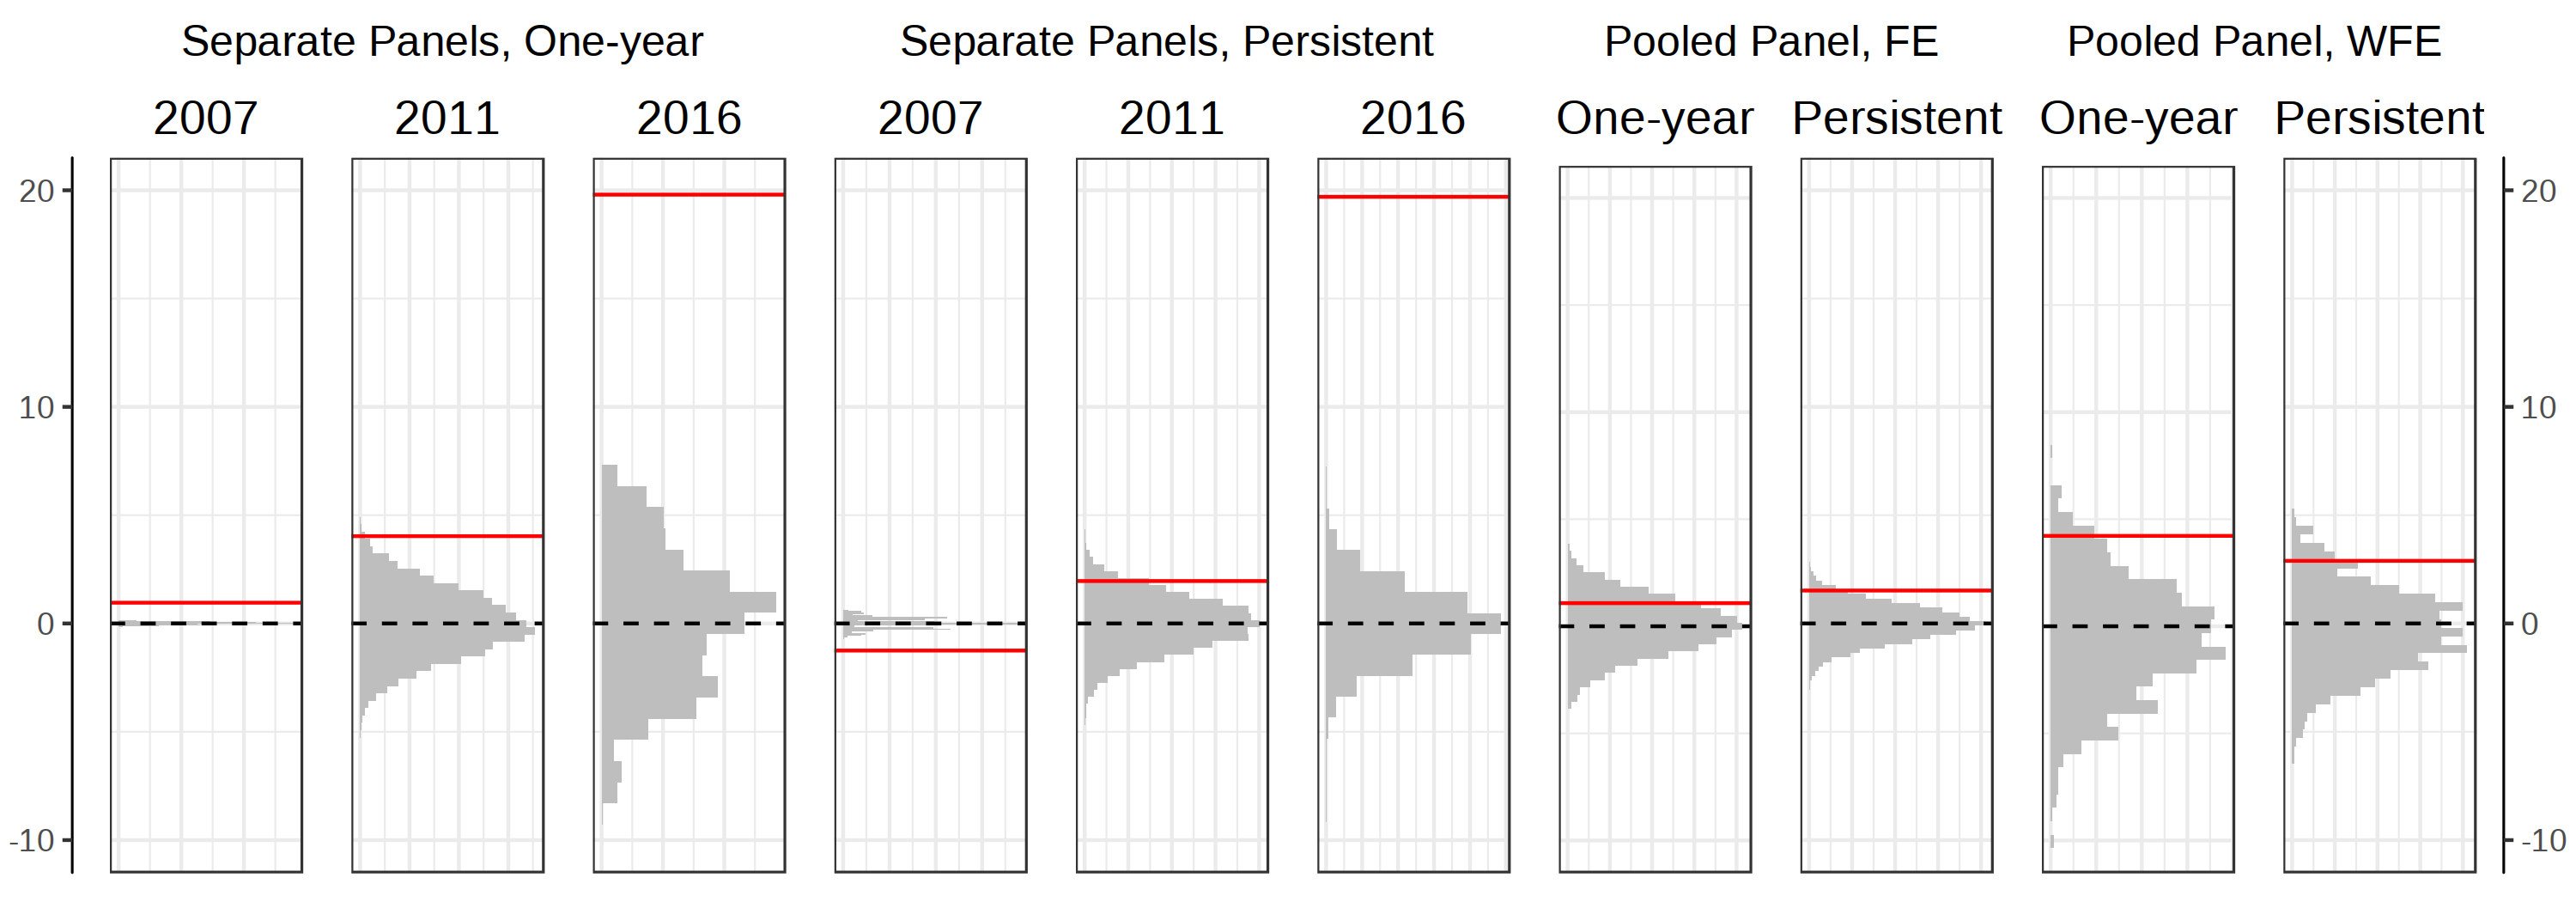
\includegraphics[width=\textwidth]{figure/SYP_FE.png}
	\captionsetup{singlelinecheck=off}
	\caption[Estimated treatment effects for linear unit fixed effects models]{Estimated treatment effects (red) and randomization distribution for linear unit fixed effects models.}
		\label{fig:FE}
	\end{figure}

Among the results, the FE and WFE pooled panel estimates carry the most weight, since they make full use of the panel structure of the data. These estimates suggest a positive and statistically significant treatment effect. In other words, they show that, on average, provinces that suffered local defeats received increases in central transfers. This evidence is supportive of the theory that the CPV uses election to gather information on the geographic distribution of regime support, and interprets local defeats to be a symptom of declining support that necessitates placation.

Estimates for the contemporaneous and for persistent effects are very close to each other (with the exception of those for the 2007 election, which uses only one pre-treatment period), suggesting that the increase in central transfers is quite stable. This pattern is also consistent with the ``geographic distribution'' theory. Indeed, if the regime uses elections to know about the level of support in individual provinces, the only way for it to know if the buying off strategy works is to wait until the next election; until then the regime must maintain a steady flow of transfers to the province.  If instead the regime uses elections to learn about individual bureaucrats' performance, the information from elections would soon be diluted by other sources of info that the regime has, including future interactions between provincial leaders and central leadership. The bureaucrats would also have opportunity to redeem themselves by performing well in other areas. This would result in a decreasing need for the regime to maintain its initial policy, which will show up in the analysis as a smaller persistent effect compared to the contemporaneous effect.

On the other hand, estimates using separate panels vary greatly from one panel to another. This suggests that the treatment effect may vary across elections, with local defeats in later elections inviting much more intense response from the CPV. Alternatively, provinces with local defeats in 2016 may differ from provinces with local defeats in 2011 and 2007 in ways that influence the magnitude of treatment effect. There is concern that the pooled estimates may be driven by the very large estimates for 2016, but it remains true that estimates for 2007 and 2011 are also mostly positive.

\subsection{Placebo tests and robustness checks}

\begin{figure}[!htbp]
	\centering
	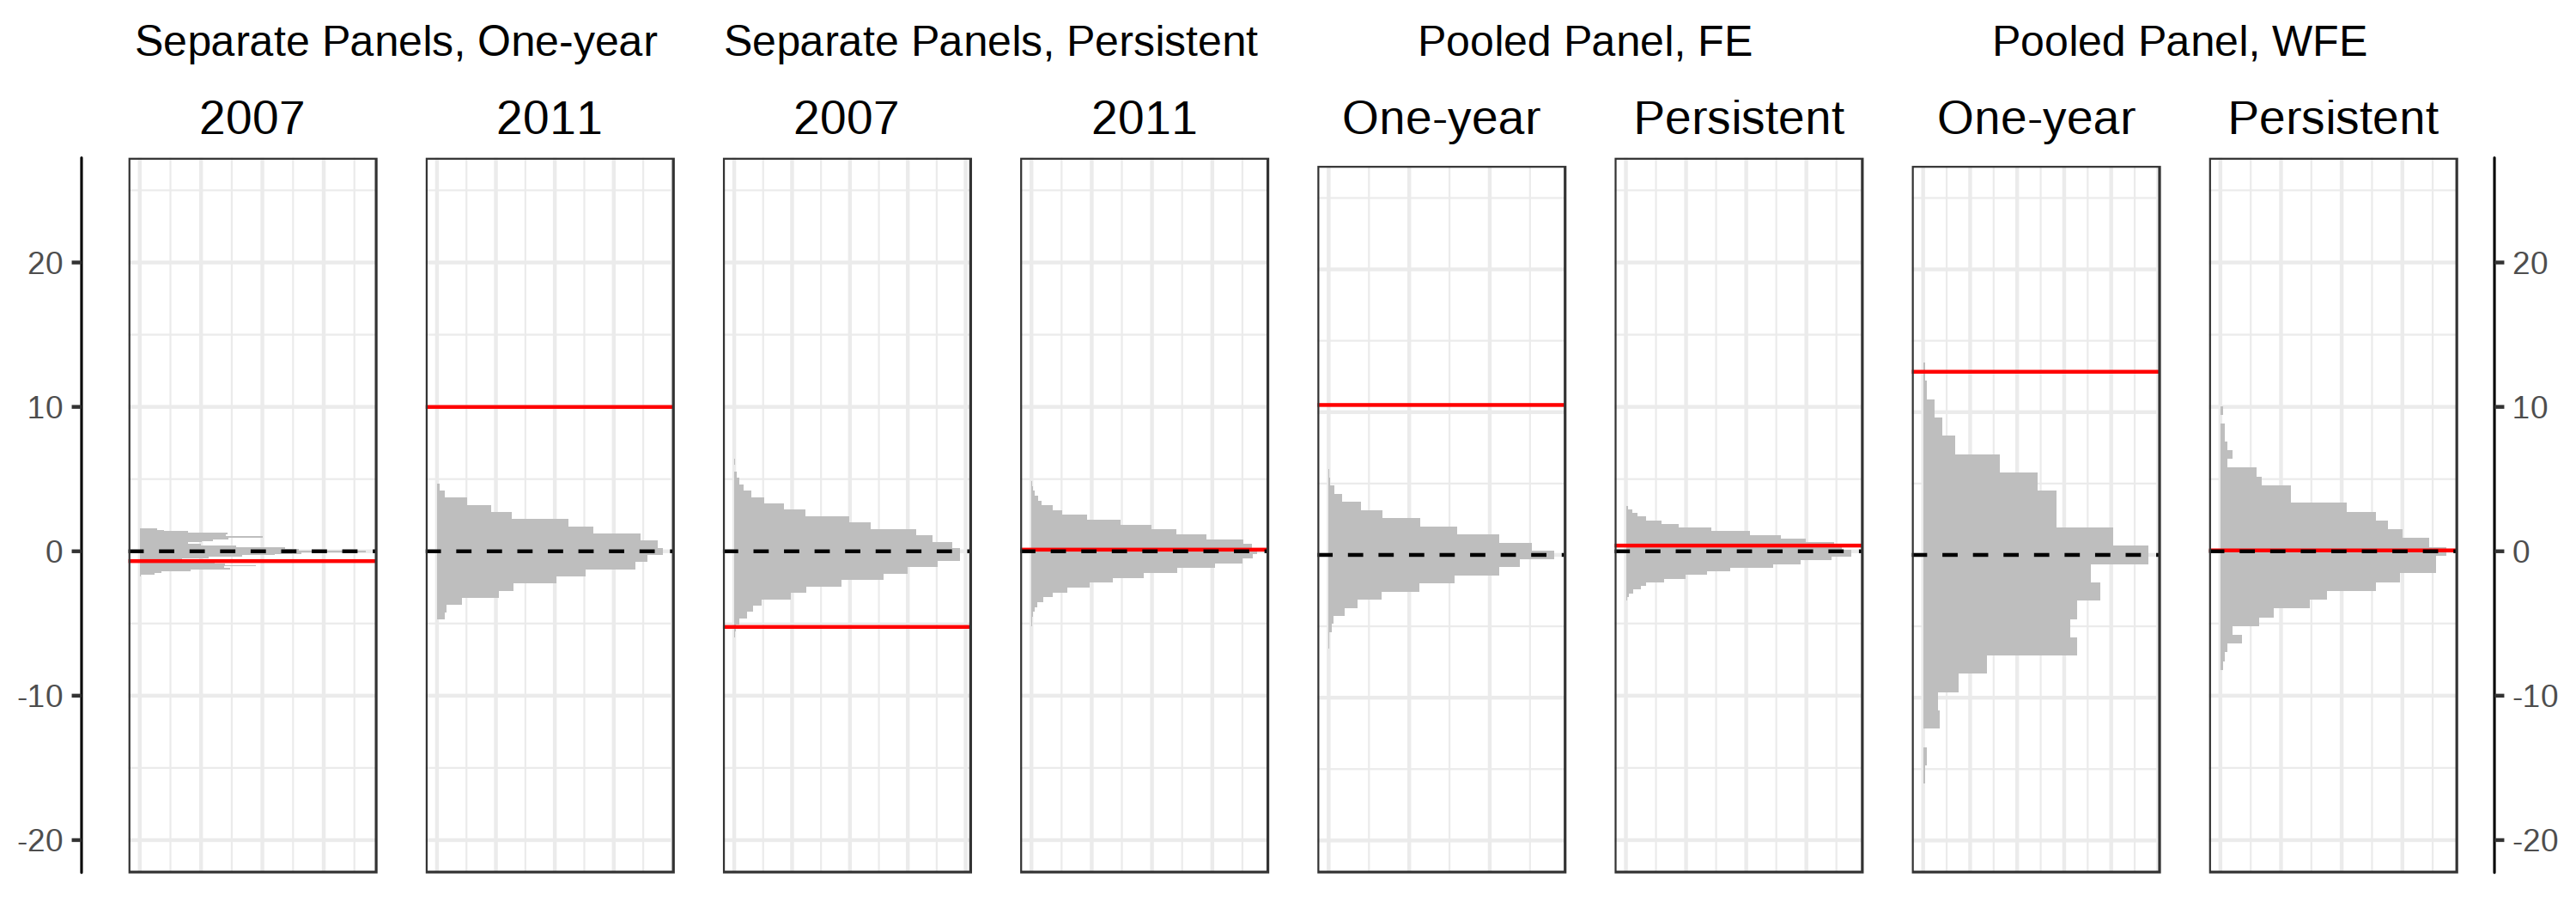
\includegraphics[width=\textwidth]{figure/SYP_FE_PLACE.png}
	\captionsetup{singlelinecheck=off}
	\caption[Estimated effects of future treatment]{Estimated placebo treatment effect (red) and randomization distribution for linear fixed effect models using local defeats in the next election as treatment.}
	\label{fig:Place}
\end{figure}

I conduct several placebo tests to verify the validity of this paper's research design. Figure \ref{fig:Place} shows one such tests, done by analyzing the effect of the \text{future} election on present. In the absence of dynamic causality, the few significant results in Figure \ref{fig:Place} would imply serious flaws in the design, since it should not be possible for a treatment in the future to impact outcomes in the present. However, in the context of this paper, they are likely indicators of dynamic causal relationships; most probably they show that present outcomes may influence future treatments, or that present treatments may influence future treatments through present outcomes. Another placebo test looking at the effect of present treatment on past outcomes in non-election years (not shown) shows similar results. In both tests, the problem seems to be more serious for estimates of contemporaneous effects than it is for persistent effects.

The apparent dynamic causality necessitates the synthetic control method. Figure \ref{fig:Synth} shows the estimated treatment effects for the synthetic control estimate for the 2016 election, along with two placebo tests that look at difference in outcomes one and two year prior to treatment -- as if the election took place in 2015 and 2014 instead. The effect of the true treatment is positive and lies far enough to the tail of the randomization distribution, which is consistent with results from the linear fixed effects regressions. Even more assuring, the placebo tests show estimates that are much closer to zero and lies further inside the randomization distribution, suggesting that the synthetic control method does indeed mitigate the problem of dynamic causality.

\begin{figure}[!htbp]
	\centering
	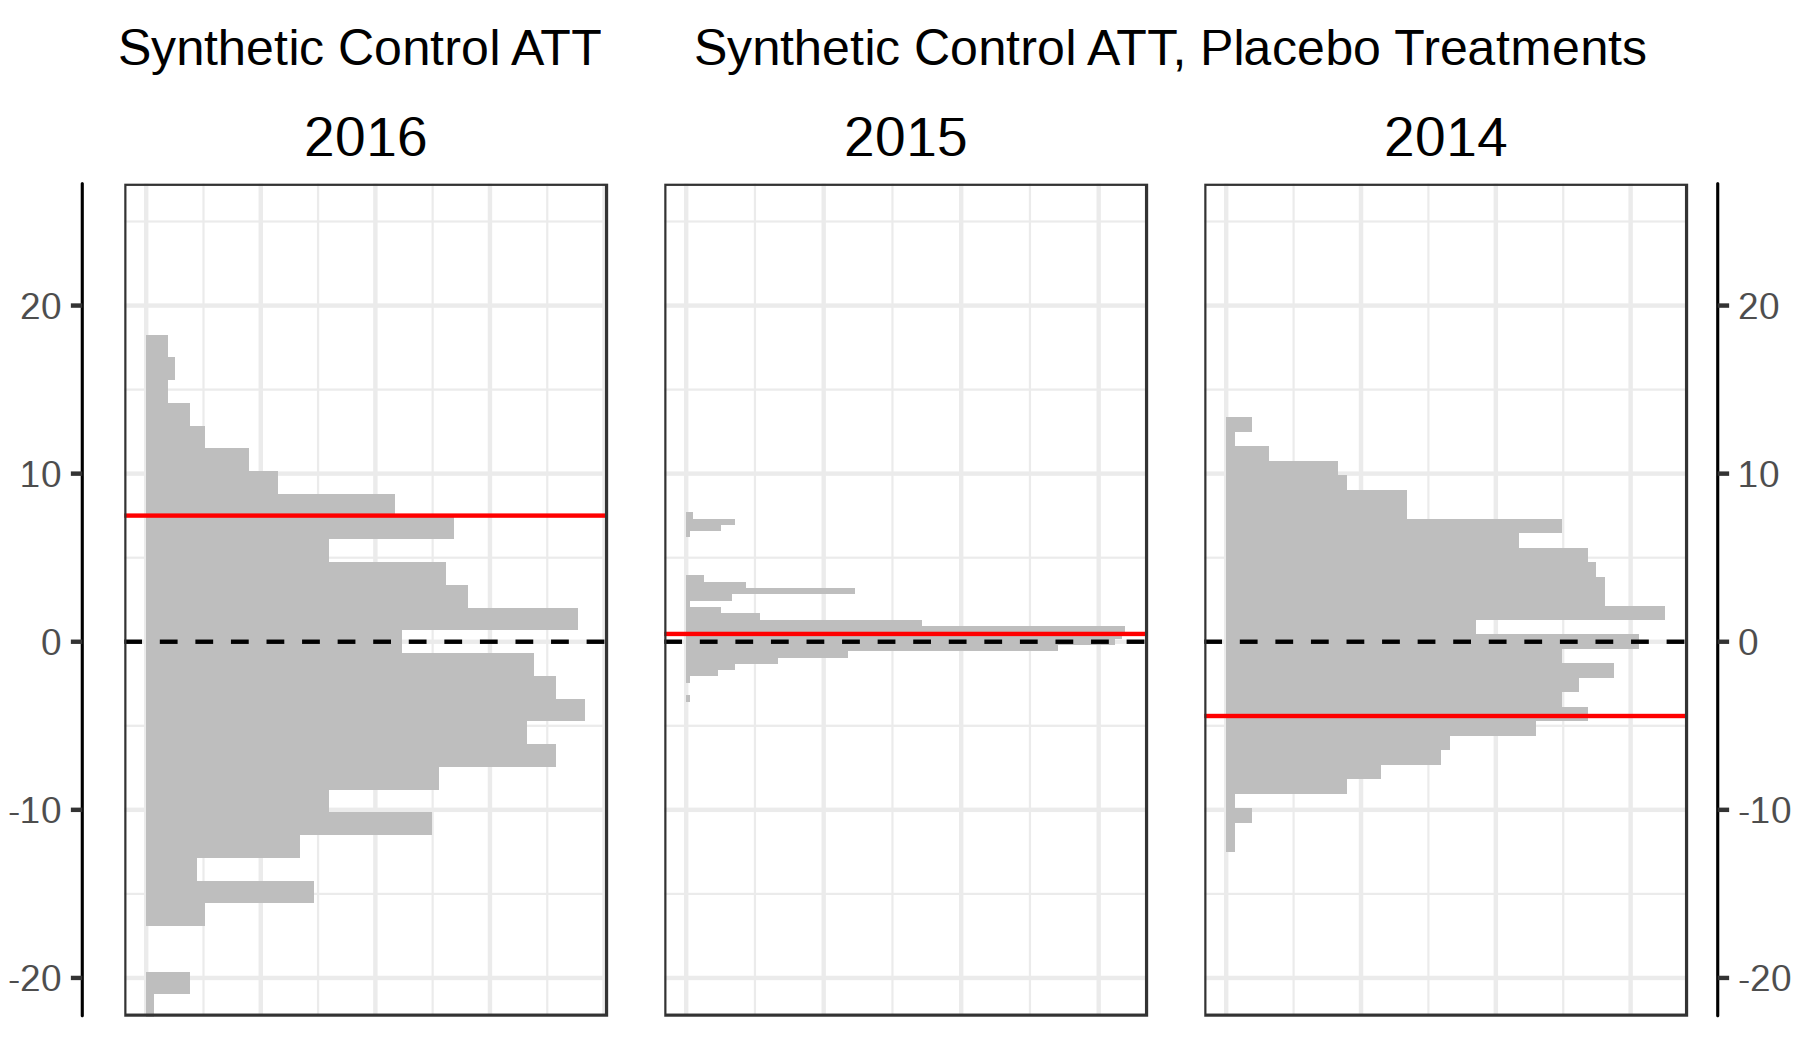
\includegraphics[width=\textwidth]{figure/SYP_Synth.png}
	\captionsetup{singlelinecheck=off}
	\caption[Estimated treatment effects for Synthetic Control]{Estimated treatment effect (red) and randomization distribution for synthetic control estimate for the 2016 election.}
	\label{fig:Synth}
\end{figure}

It is necessary to point out that, for the 2016 election alone,\footnote{This is the only election for which the pre-treatment period is long enough.} the point estimate using the synthetic control method differs from both the equivalent fixed effects estimates. The difference in magnitude is roughly 12 points on the log scale, roughly .6 of the fixed effects estimates. This discrepancy highlights potential violation of the causal assumptions, either on the part of the fixed effects model or the synthetic control method, a problem I noted earlier. Considering, however, that both estimates are strongly positive and significant, it is unlikely that violation of either causal assumptions would invalidate the main conclusion of this analysis.

For robustness checks, I repeated the above analyses using an array of modified specifications.\footnote{I do not show these results in the interest of space.} To begin with, I vary the size of the control sets by using alternative vote share thresholds for close wins at 55 and 65 percentage points. This results in noisier estimates, but the direction of the findings remains consistent, especially for the four models using pooled data. Additionally, I include as an additional control to every model an average of central nominees' strength. It is calculated following a formula by \cite{MaleskySchuler2011}, by summing indicators for whether the candidate is a member of the local legislature, the local party secretariat, the local people's committee, the CPV's Politburo, the CPV's central committee, or the outgoing NA. The strength of central nominees is likely to have been a determinant of their election prospects, but I am not confident that this formula correctly captures these candidates' strength \textit{as seen by the voters}, and so have relegated this variable to a robustness check instead of including it in the main models. In any case, controlling for central nominee strength has virtually on impact to the main results. This is probably because the remaining controls have fully captured most variation in the CPV's pre-election manipulations.

\subsection{Mechanism}

\begin{figure}[!htbp]
	\centering
	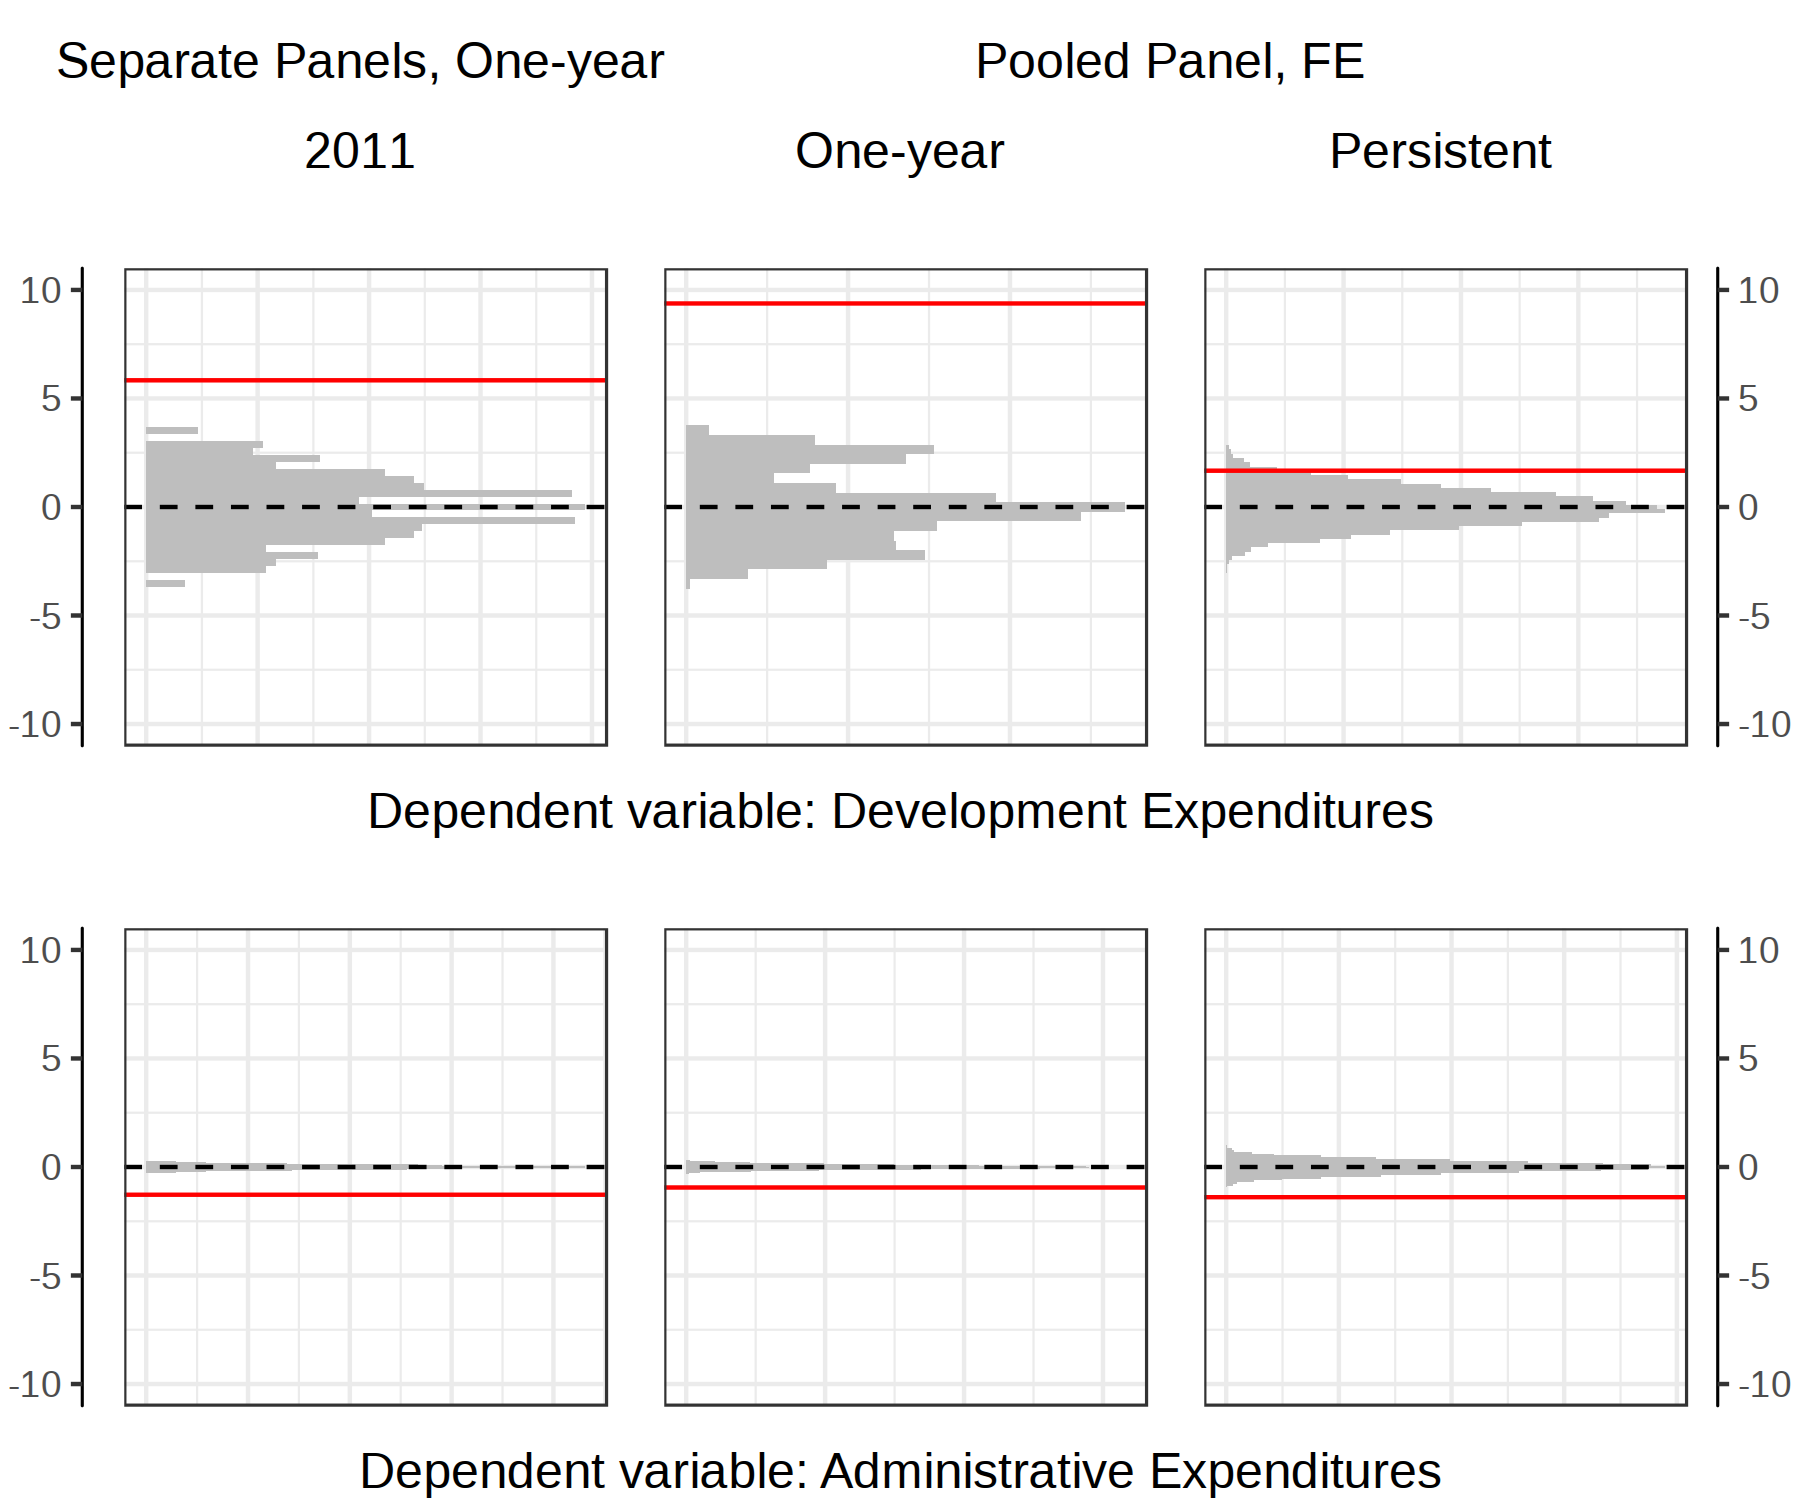
\includegraphics[width=\textwidth]{figure/SYP_FE_MECH.png}
	\captionsetup{singlelinecheck=off}
	\caption[Estimated effects of future treatment]{Estimated treatment effect (red) and randomization distribution for linear fixed effect models using local defeats in the next election as treatment.}
	\label{fig:Mech}
\end{figure}

The main results from the linear fixed effects regressions have found that the CPV increases central transfers to provinces that witnessed local defeats of central nominees. According to the ``geographic distribution'' theory of authoritarian elections, such increased transfers would be spent on public projects that would placate the local publics, as opposed to being used as a source of graft. Figure \ref{fig:Mech} tests exactly this for the subset of regressions for which data is available.\footnote{Province-level budget data is not available for 2016, and has high incidence of missingness for earlier years} It shows the treatment effects of local defeats on two components of province-level expenditures. The first row shows the treatment effect on investment in developmental projects, and the second row shows the treatment effect on administrative expenditures. The analysis shows some suggestive evidence that local defeats lead to increase in investment in developmental projects and a small decrease in administrative expenditures, which is consistent with the ``geographic distribution'' theory.


\subsection{Alternative Explanations}

\subsubsection{Both theories may hold}

\begin{figure}[!htbp]
	\centering
	\begin{subfigure}[!htbp]{\linewidth}
		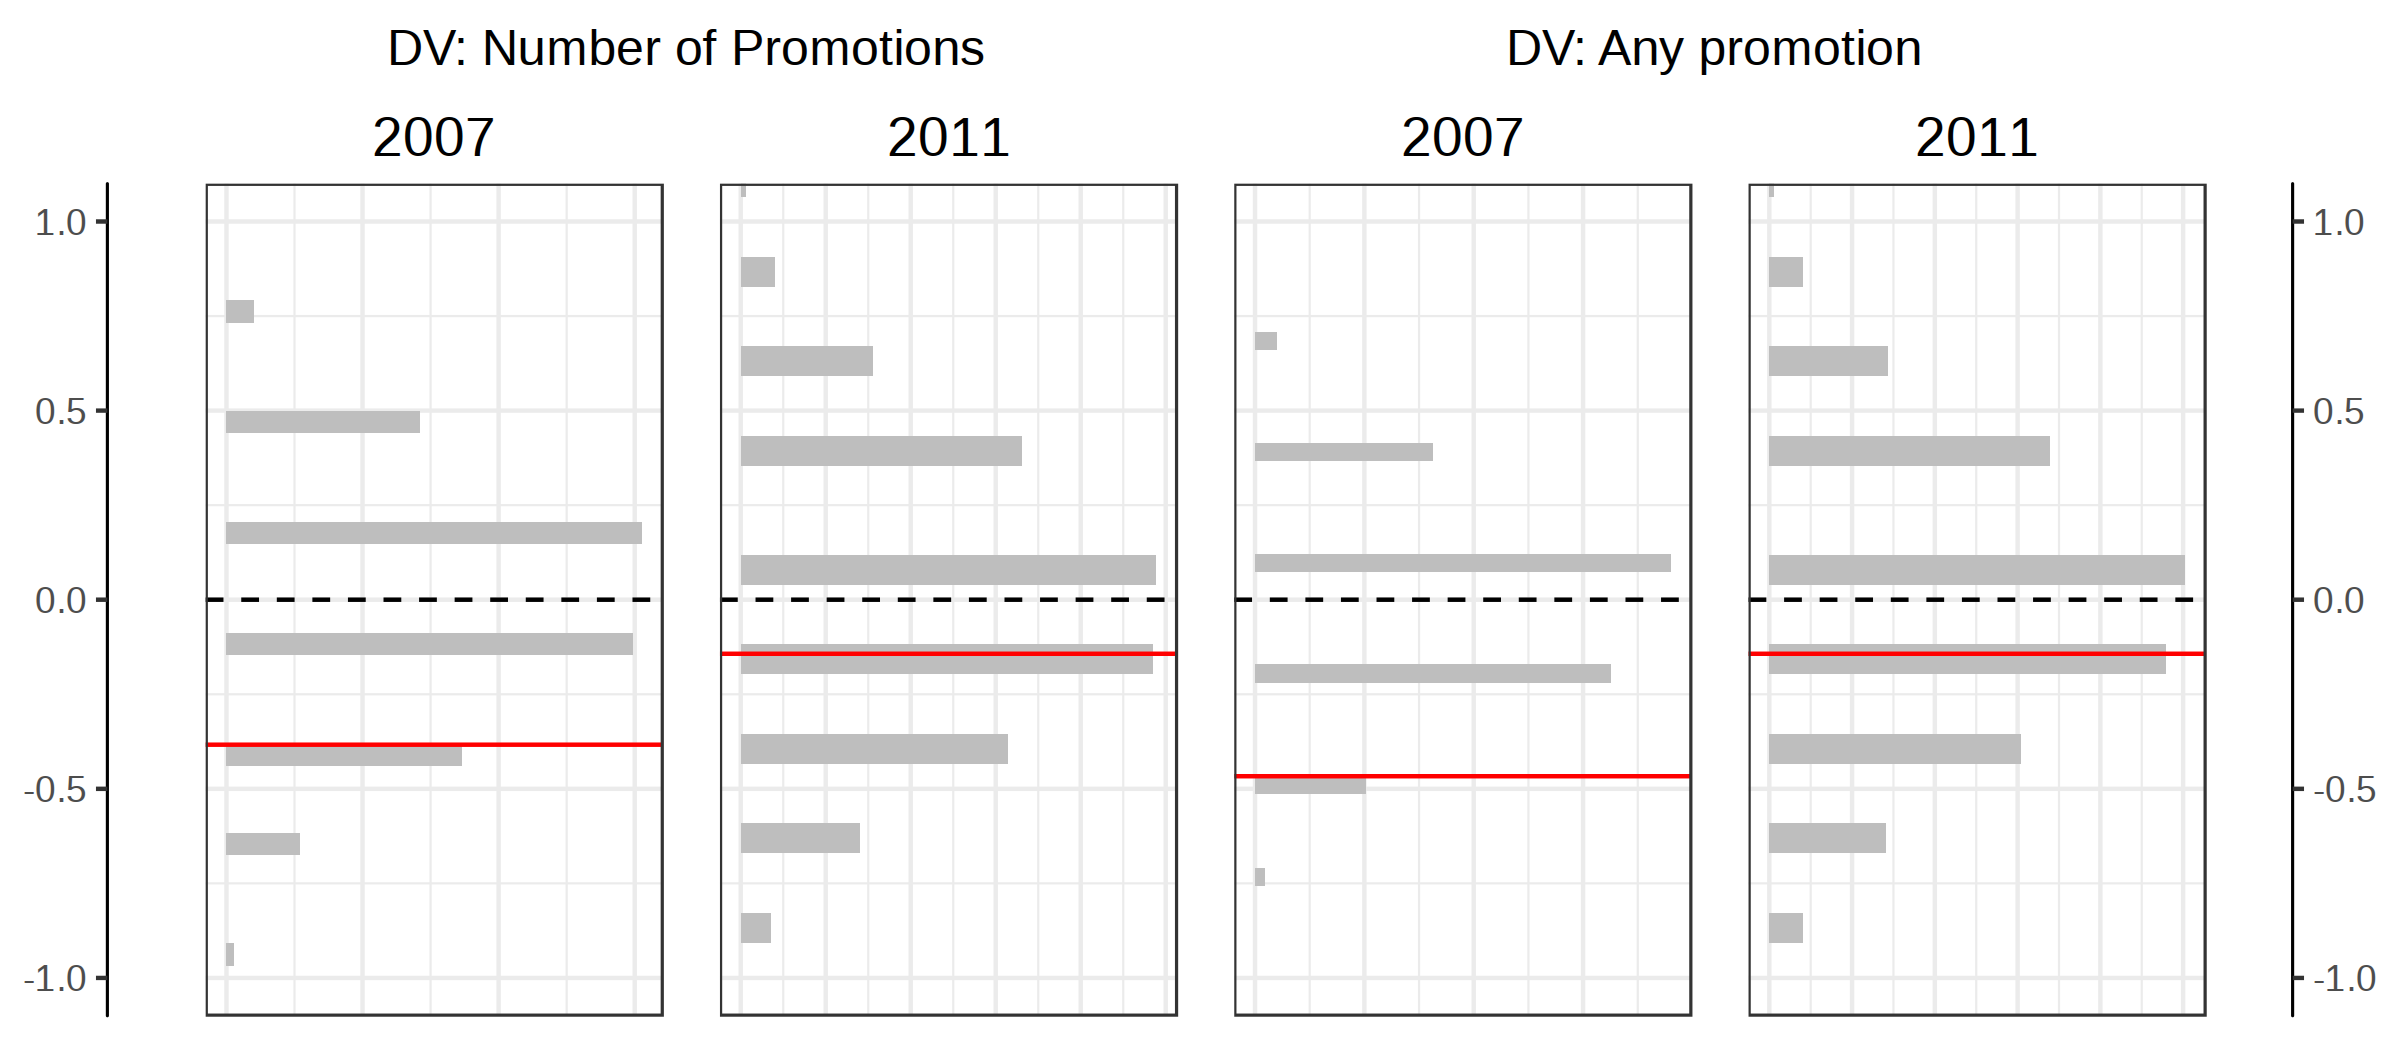
\includegraphics[width=\textwidth]{figure/SYP_RI_LEAD.png}
		\caption{Governing \textit{during} election years}
		\label{fig:Lead}
	\end{subfigure}
	
	\begin{subfigure}[!htbp]{\linewidth}
		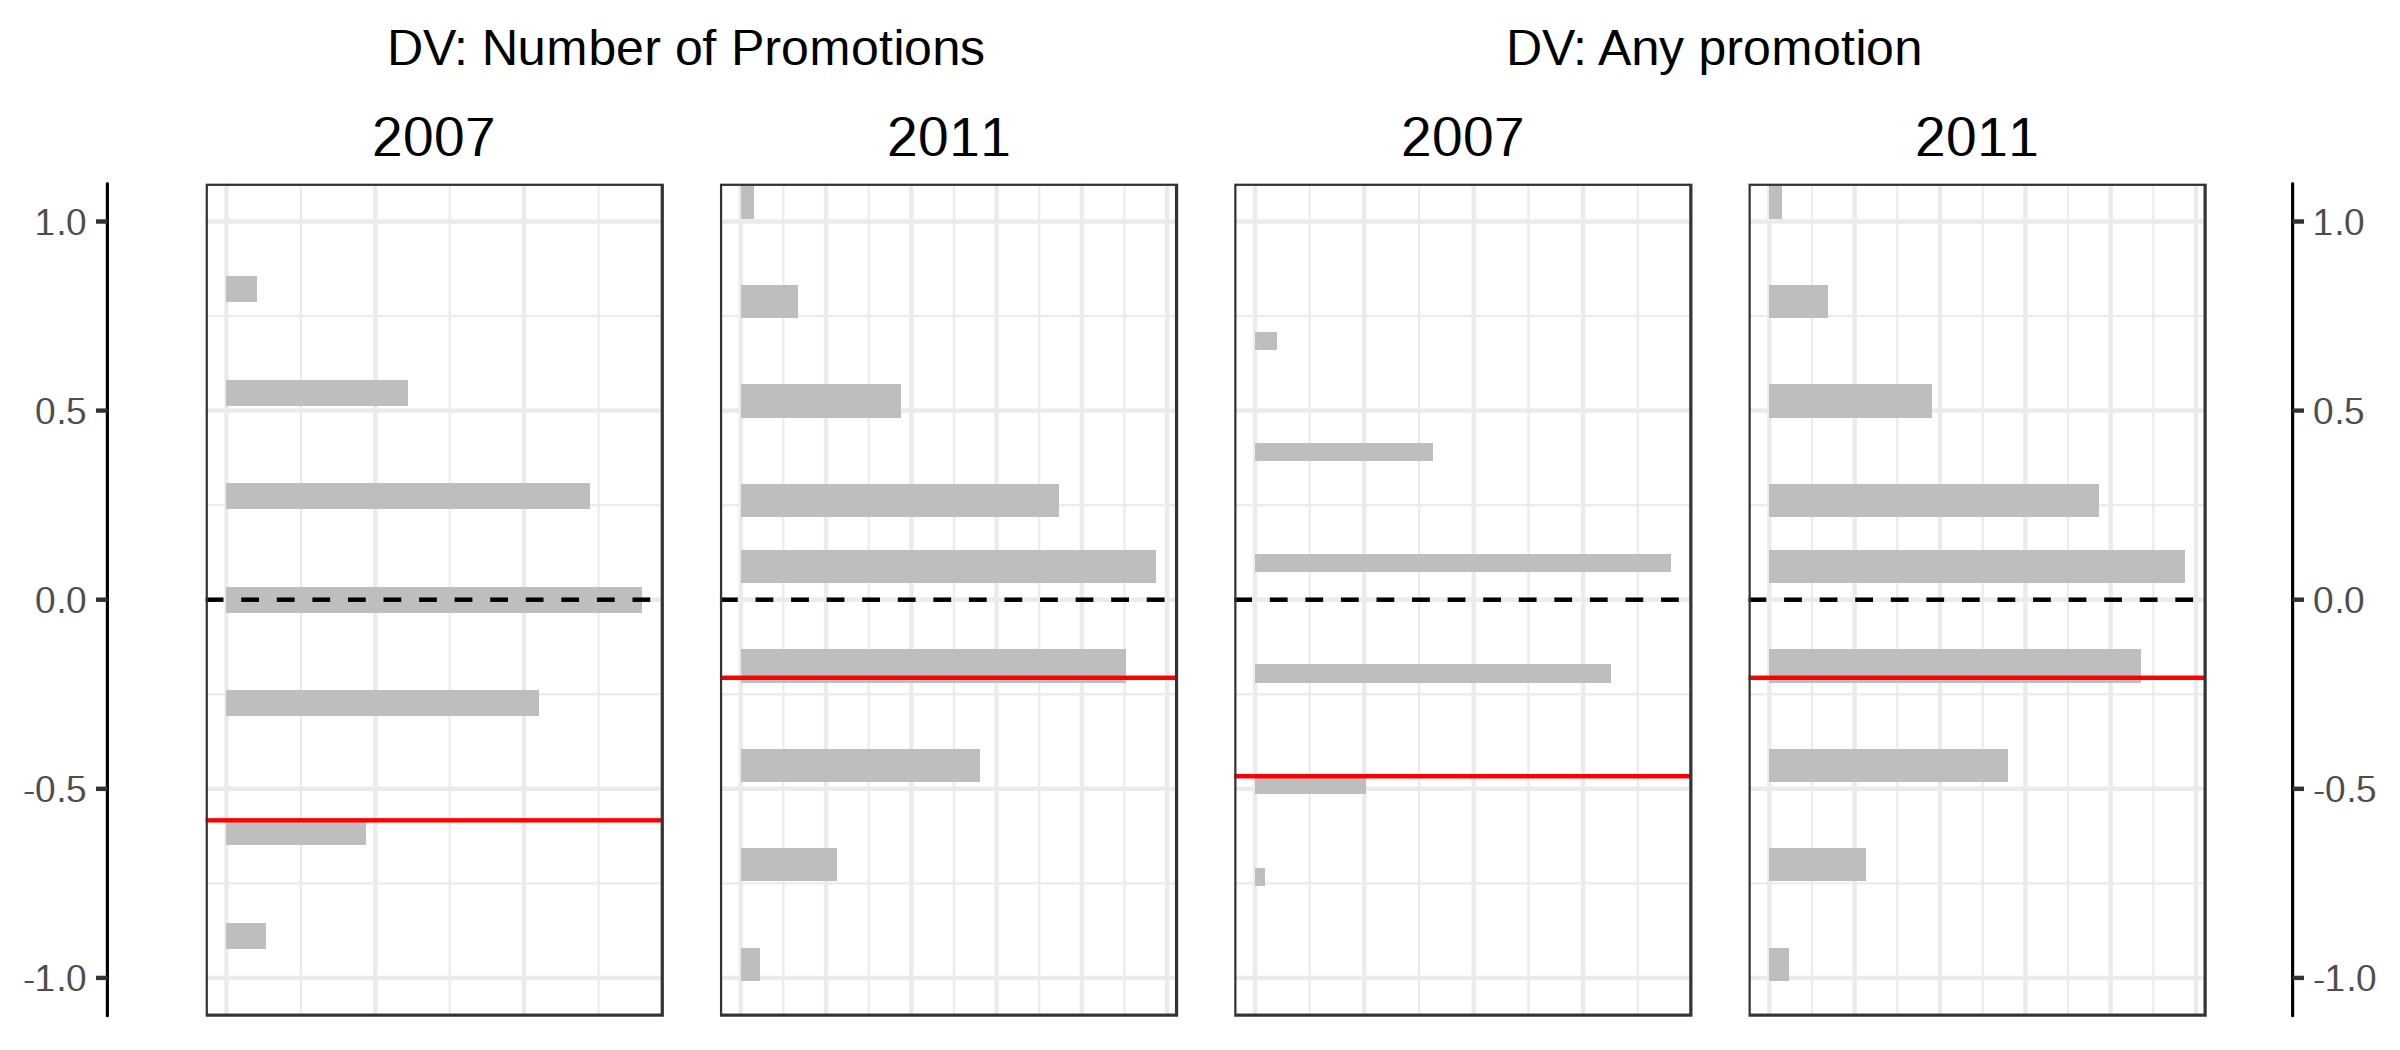
\includegraphics[width=\textwidth]{figure/SYP_RI_LEAD_LAG.png}
		\caption{Governing \textit{before} election years}
		\label{fig:Lead_Lag}
	\end{subfigure}
	\caption[Estimated treatment effects of on promotion]{Estimated effect (red) of local defeats on promotion prospects of top provincial bureaucrats and randomization distribution for comparison-of-means estimates. The estimates for 2007 lie far towards the tail of the distribution, but not enough to cross the $p=0.1$ threshold.}
\end{figure}

Even with the evidence that local defeats lead to increased transfers, it is still possible to defend the ``local bureaucrats'' theory by arguing that the regime sees election defeats as providing \textit{both} types of information, but uses different response tools to act on each information. In section \ref{sec:vs} I have argued that this is not likely, because the regime does not have many response options other than through the budget channel. Even the most straightforward option -- directly sanctioning bureaucrats by firing, demoting, or delaying promotion -- is not appropriate given the leadership shuffling schedule and the need of the party to project an image of unity. I verify this argument using a dataset on career of top provincial bureaucrats from 1991 to 2015 offered by \cite{MaleskyPhan2017}.\footnote{For each province, the top provincial bureaucrats are the Secretary of the Provincial Party Committee and the Chairman/Chairwoman of the People's Council. The first position is the head of the party in the province, and the second position is the head of the government, similar to a mayor.} The data shows that, between 2005 and 2015, with only extremely rare exceptions, there have been virtually no firing or demotion happened to provincial leaders. The evidence on delayed promotion is similarly thin. Figure \ref{fig:Lead} shows that the impact of local defeats on the promotion of provincial leaders between the year after one election and before the next, as estimated by a simple comparison of means between treated and control units within the subset sample,\footnote{Since the data is collapsed into cross-sections rather than panels, there are not sufficient degrees of freedom to control for covariates.} is close to zero and lies far inside the randomization distribution. The same results hold for both the number of promotions in the period, as well as for whether \text{any} promotion occurred. 

Another possibility is that the CPV monitors and punishes not the officials responsible for managing the elections, but those running the province prior to the elections. Recall that top provincial bureaucrats in Vietnam are transferred into a province just before an election, and are then left to run the province up until just before the next election. If the party accepts that its local defeats are the result of low popularity within individual provinces, but attributes this low popularity to the officials who had been governing the province prior to the election, then its post-election response would include both placating the public in provinces it suffered defeats in \textit{and} punishing these officials. Under this scenario, not only would both the two theories hold, but my interpretation of the NA elections as a mechanism for bottom-up accountability would also be undermined.\footnote{I thank Andy Halterman for raising this important alternative interpretation of my main results.} Reassuringly, repeating the above analysis on the career prospects of bureaucrats who served in provinces with local defeats the year \textit{just before} each election yields no evidence of punishment. Indeed, Figure \ref{fig:Lead_Lag} shows nearly identical results to those in Figure \ref{fig:Lead}. This implies that top officials in provinces that suffered local defeats, either during or right after their tenure, do not experience delayed promotion when compared to their peers in other provinces.


\subsubsection{Both theories may be wrong}

The evidence so far may also be consistent with a theory that rejects both the ``geographic distribution'' and ``local bureaucrats'' theories such as that by \cite{Geddes2005}, which posits that authoritarian regimes hold elections only so that they can secure and boast about landslide wins. As implied by this theory, the central government increase central transfers to provinces with defeats only to ensure it can manage better the next election. If this explanation is true, we should also expect other forms of electoral manipulation at the highest levels. Because the heavy-handed manipulations needed to ensure such landslide wins may obfuscate the signal from the election results, this explanation, if true, would go against all ``information flow'' theories in general.  To test this conjecture, in Appendix \ref{app:benford} I perform digit tests based on Benford's Law using publicly available election results from the 2011 and 2016 elections, and find no clear evidence of manipulation.\footnote{\cite{MaleskySchuler2011} already performed similar tests for data from 2007 election, and also found no evidence of manipulation. I successfully replicated their findings, and then extend them to the 2011 and 2016 elections.} Although the absence of implicating evidence does not completely exonerate the CPV, it suggests that either the CPV does not manipulate election results, or that all the manipulation that occurred only occurred at lower levels, perhaps without knowledge of the highest leaders.\footnote{It also rules out the scenario that the CPV collects evidence from real election results, then manipulates only the publicized results to benefit from both information and the ``show of strength.'' Had this scenario been true, publicized results would not have been an accurate measure of the information the regime receives, which invalidates any conclusion from the regression results.} In either case, the evidence contradicts with \cite{Geddes2005}'s theory: the CPV leadership does not seem to focus only on winning elections.

\section{Conclusion}
\label{sec:conclusion}

In this paper, I analyze changes in central transfers between the national government and provinces in Vietnam following three legislative elections in 2007, 2011, and 2016. Using various estimation methods to achieve causal identification, I found significant and robust evidence that the defeat of one or more central nominee(s) in a province leads to an increase in central transfers to that province. This pattern of response to local defeats is consistent with the ``geographic distribution'' theory of authoritarian election, according to which authoritarian regimes use elections to gather information about subnational variation in support for the regime. In the case of Vietnam, the empirical finding fits the ``geographic distribution'' theory's prediction that the regime perceives provinces with central nominee defeats as areas with particularly low level of support, and uses central transfers to increase public goods investment there as a means of placating the public.

This paper may justifiably attract some criticisms, but although warranted they do not entirely invalidate my findings. One potential objection is that its results and conclusions may not be perfectly generalizable to other authoritarian regimes beyond Vietnam. What this paper also shows, however, is a process to identify among the many theories of authoritarian elections ones that are most applicable to each individual context. The findings of this paper may be specific to its scope conditions -- strong institutionalized single-party regimes such as Vietnam -- but the framework can be generalizable to other contexts. In particular, researchers only need to connect each theory of authoritarian elections with the corresponding interpretations that regime leaders may have for election upsets, and, depending on the regime context, identify the logical regime responses to these interpretations. As long as there are responses that are uniquely predicted by one theory but not another, or responses that are contradictory to each other, empirically evaluating which regime responses end up being pursued will help filter out theories that are not applicable to the context. A joint effort by researchers repeating this exercise in various different regime contexts will then produce a complete mapping of which theory applies to which set of scope conditions, filling in the gap in the literature.

Moreover, even this paper's specific conclusions may apply to a broader than expected range of cases. Not only do they apply to strong communist states like Vietnam and China, but these conclusions may also be anticipated in every regime where a ruling party is a) dominant enough to not worry about the threat of organized opposition to its prospect of election victory, b) has centralized control over public finance distribution to subnational units. A number of cases may fit this description, including Singapore under the PAP, Malaysia under the UMNO, Japan under the LDP, and even -- at the height of the ruling parties' power -- Mexico under the PRI and Egypt under the NDP, subjects of the two studies that motivated this paper \citep{Magaloni2006, Blaydes2008}. In all these cases, whether the regime has reliable alternatives to gauge the competence and loyalty of its subordinates such as it does in Vietnam is likely to determine whether election is used to monitor the geographic distribution of support instead of local bureaucrats.

In terms of empirics, critiques may draw attention to the large variation in the estimates of the causal effects, as well as evidence of causal identification violations that neither of my two empirical methods have fully addressed. This is an almost inevitable problem of causal inference with non-experimental data. However, the various adjustments, robustness checks, and tests of auxiliary outcomes together do produce quite consistent results, which lends confidence if not to the point estimates then to the general directions of the findings.

Ultimately, given the modest goals it seeks to achieve, this paper does make some contribution to the larger literature. It contributes to the ``information flow'' literature of authoritarian institutions by attempting to specify the exact kind of information that authoritarian regimes collect through elections. In doing so, I evaluate two theories with potentially contradictory implications, and develop a procedure to test their validity as applied to a specific context. Throughout this paper, I conceive of authoritarian leaders as imperfect optimizers who consciously seek information to update their beliefs and modify behaviors accordingly, but are predisposed to interpret the information they receive in certain ways. This perspective could contribute to the broader literature on authoritarianism, which has mostly portrayed regime leaders as rational actors \citep[e.g.][]{AR2001}, by bridging it with the recent literature on political behavior which has begun to highlight the imperfect psychology of individual citizens \citep[e.g.][]{AchenBartels2016}. In addition, to the literature on accountability in authoritarian regimes, it recommends a rethinking of even uncompetitive elections as a possible avenue for accountability. In particular, it shows for the case of Vietnam that, even when elections pose only non-existential threat to the regime, negative results from them can still convey to it the public's dissatisfaction, and induce it to react in a way that enhances citizens' welfare. On one hand, this suggests that autocrats can and may respond to dissatisfaction just like democrats do. On the other hand, the potential for limited accountability under authoritarian regimes provide another explanation for their durability, which in the long run may not be optimal for development outcomes.

\inputencoding{utf8}
\bibliography{Literature/library_syp}

\newpage
\appendix

\section{Next steps}
Although this is the final draft of this paper, there are several modifications and improvements I still hope to make for this paper if given a much larger amount of time and space. In this section I elaborate some of my future ideas for this paper.

\subsection{Reframing}

One major feedback I have received from discussion with my readers and others is that there are two potential directions I should take for this paper. One is to turn it into a paper about Vietnam with the explicit purpose of introducing how authoritarian elections work in this specific case. This paper would fit with an audience of regional scholars, who would appreciate the country-specific details without scrutinizing my theories too much. The other option is to write it as a general ``comparative politics of authoritarian elections'' with greater emphasis on theories and more argumentation about how the Vietnam case can be generalizable. This option would win a greater audience, but the bar for originality would be much higher.

To decide which path to follow, I am looking to find out how generalizable the Vietnam case could actually be, by identifying potential cases where similar dynamics would hold and verify that this is true. If a sufficiently large number of such cases exist then the second option would be ideal. Otherwise, limiting the paper to a smaller audience would be better. So far I have identified only a few cases, as listed in my conclusion, and am hoping to test if these cases are indeed similar to Vietnam in terms of scope conditions. This will take some time, and even then my prior is still that they are not. As a result I am prepared to limit this paper to the smaller audience. This option would conveniently require much less reframing on my part.

\subsection{Extra supporting evidence}

Even as a country-specific paper, there are several additional pieces of evidence I hope to collect, namely:

To verify that the observed outcomes actually reflect planned action i.e. that the central government intentionally increases transfers to provinces with local defeats, I hope to directly confirm with government officials. The best would be to talk to retired officials. Additionally I can conduct survey experiments with local bureaucrats at provincial or just-below-provincial levels to inquire what they think would happen to provinces with local defeats. Although the regime does not publicly discuss this information, I expect it to be more or less acknowledged among party bureaucrats. Thus if survey experiments with bureaucrats show some level of consensus I would be much confident in my findings.

To verify that there is indeed no punishment of provincial bureaucrats in provinces with local defeats, I hope to look at a broader range of outcomes, such as:
\begin{itemize}
	\item Investment in SOEs, which can be a very probable source of graft
	\item Investment in the construction of monuments or government buildings, which brings no particular benefits to the public but can be a source of graft for government officials
	\item Instances of central party leaders making appearances at provinces, which can be acquired by scraping official news outlets, and which signifies close relationships between central and local officials	
\end{itemize}

To verify that central transfers to provinces are indeed intended to placate the public, I hope to look at end-outcomes that are more relevant for the public, such as:
\begin{itemize}
	\item Local level public goods, which can be obtained in the commune-level Vietnam Household Living Standards Survey. I currently have access to the 2002, 2004, 2006, 2008, 2010, and 2012 waves of the survey, and just need to collect the 2014 and 2016 as well as waiting for the future 2018 waves.
	\item Local level governance quality, which can be obtained through the Provincial Administration Performance Index (PAPI) and Provincial Competitiveness Index (PCI) collected by Eddy Malesky.
\end{itemize}

\subsection{Incorporating with other research}
Once I have collected sufficient additional evidence and have decided on an appropriate framing for the paper, I am hoping to submit it to an appropriate journal, and then incorporate it into my larger dissertation research. One way is to use the paper as one chapter in a book project, like how Rory Truex did for Chapter 6 of his recent book \citeyearpar{Truex2016}. As of right now, I am planning for my dissertation to be about ``unintended'' forms of accountability under authoritarian regimes, so this paper would fit nicely as one case study.

\newpage
\section{Linear fixed effects regression using first-differenced outcomes as triple-differences}
\label{app:proof1}

Let $T_{it}$\footnote{I'm still working on this section, and currently is abusing notation a bit} be an indicator of treatment status in every period such that $T_{it} = 1$ for treated provinces and for every year, $E_{it}$ be indicator for sample, such that $E_{it} = 1 $ for unit-year that may be exposed to treatment and $E_{it} = 0$ for placebo units, $G_{it}$ be indicator for post-treatment periods,, the normal difference-in-difference is given by:
	\begin{align*}
		& \l[\E[Y_{i,t} | T_{it}=1, G_{it}=1, E_{it}=1] - \E[Y_{i,t} | T_{it}=1, G_{it}=0, E_{it}=1]\r] \\
		&\phantom{=} - \l[\E[Y_{i,t} | T_{it}=0, G_{it}=1, E_{it}=1] - \E[Y_{i,t} | T_{it}=0, G_{it}=0, E_{it}=1]\r]
	\end{align*}
The placebo difference-in-difference is given by:
	\begin{align*}
		&\l[\E[Y_{i,t} | T_{it}=1, G_{it}=1, E_{it}=0] - \E[Y_{i,t-1} | T_{it}=1, G_{it}=1, E_{it}=0]\r] \\
		&\phantom{=} - \l[\E[Y_{i,t} | T_{it}=0, G_{it}=0, E_{it}=0] - \E[Y_{i,t-1} | T_{it}=0, G_{it}=0, E_{it}=0]\r]
	\end{align*}
When estimated separately, each difference-in-difference can be estimated using fixed effects regression with the outcomes $Y_{i,t}$ in the left hand side.

Now assuming that treatment takes place in year $t$, so the normal difference-in-difference becomes:
	\begin{align*}
		& \l[\E[Y_{i,t} | T_{it}=1, E_{it}=1] - \E[Y_{i,t-1} | T_{it}=1, E_{it}=1]\r] \\
		&\phantom{=} - \l[\E[Y_{i,t} | T_{it}=0, E_{it}=1] - \E[Y_{i,t-1} | T_{it}=0, E_{it}=1]\r]
	\end{align*}
The placebo difference-in-difference is then 
	\begin{align*}
		& \l[\E[Y_{i,t'} | T_{it'}=1, E_{it'}=0] - \E[Y_{i,t'-1} | T_{it'}=1, E_{it'}=0]\r] \\
		&\phantom{=} - \l[\E[Y_{i,t'} | T_{it'}=0, E_{it'}=0] - \E[Y_{i,t'-1} | T_{it'}=0, E_{it'}=0]\r]
	\end{align*}
with $t'$ being any year outside of the election cycle.

The difference-in-differences-in-differences will then be:
	\begin{align*}
		&\phantom{=}\bigg[\l[\E[Y_{i,t} | T_{it}=1, E_{it}=1] - \E[Y_{i,t-1} | T_{it}=1, E_{it}=1]\r] \\
		&\phantom{=} - \l[\E[Y_{i,t} | T_{it}=0, E_{it}=1] - \E[Y_{i,t-1} | T_{it}=0, E_{it}=1]\r]\bigg] \\
		&- \bigg[\l[\E[Y_{i,t'} | T_{it'}=1, E_{it'}=0] - \E[Y_{i,t'-1} | T_{it'}=1, E_{it'}=0]\r] \\
		&\phantom{=} - \l[\E[Y_{i,t'} | T_{it'}=0, E_{it'}=0] - \E[Y_{i,t'-1} | T_{it'}=0, E_{it}=0]\r]\bigg] \\
		& = \l[\E[\Delta Y_{i,t} | T_{it}=1, E_{it}=1] - \E[\Delta Y_{i,t} | T_{it}=0, E_{it}=1]\r] \\
		&\phantom{=} - \l[\E[\Delta Y_{i,t'} | T_{it'}=1, E_{it'}=0] - \E[\Delta Y_{i,t'} | T_{it'}=0, E_{it'}=0]\r]
	\end{align*}	
which is a difference-in-differences using first difference and change scores.

\newpage
\section{Digit tests showing no evidence of high-level manipulation}
\label{app:benford}
To verify that the CPV does not engage in overt \textit{ex-post} manipulation of vote results at the high level (for example by changing the vote tallies), I conduct several digit tests on publicly-available vote results from the 2011 and 2016 elections. 

Digit-based tests have been used widely in the election forensics literature to detect evidence of fraud both in American \citep{Mebane2006} and Comparative Politics \citep{Mebane2009, Beber2012}. Many of these tests are based on Benford's Law, which states that digits in naturally occurring numbers follow certain patterns, and that human interventions in the data generation process can lead to violation of these patterns. Because many numbers produced in an elections such as vote counts or turnout figures are naturally occurring numbers, they can be tested against the patterns to detect suggestive evidence of human tampering \citep{Mebane2006}. Under the null hypothesis, Benford's Law suggests that the probability that the first $m$ digits of a number follow a particular sequence is given by:
\begin{align*}
P(D_1=d_1, D_2=d_2, \dots, D_m=d_m) &= \log_{10}\l(1 + \l( \sum_{j=1}^{m}10^{m-j}d_j\r)\r)
\end{align*}
where $D_i$ represents the $i$th significant digit, and $d_i$ is a particular realization of that digit. From this, it is possible to calculate the Benford Distribution for the First Digit:
\begin{align*}
	P(D_1=d_1) = \log_{10}\l(1 + \frac{1}{d_1}\r)
\end{align*}
as well as the Benford Distribution for the Second Digit:
\begin{align*}
	P(D_2=d_2) = \sum_{j=1}^{9}\log_{10}\l(1 + \frac{1}{10j + d_2}\r)
\end{align*}
and for the Third Digit:
\begin{align*}
	P(D_3=d_3) = \sum_{k=1}^{9}\sum_{j=0}^{9}\log_{10}\l(1 + \frac{1}{100k + 10j + d_3}\r)
\end{align*}
and so on. Note that as $i$ increases, the distribution converges quickly to uniform.

I conduct digit tests for the first three significant digits of three measures: voter turnouts in the 2011 election, number of invalid votes for the 2011 election, and candidate vote counts for the 2016 election. All three measures are recorded at the electoral district level, which is the lowest level for which data is publicly available. Unlike vote shares, which is used by \citep{MaleskySchuler2011}, none of these three are bounded above and beyond, are not subjected to rounding, and span multiple orders of magnitude, which are important requirements for Benford-like number distributions \citep{Hill1995, Mebane2006, Berger2015}.

Figure \ref{fig:Benford} shows the results, in the form of histograms showing the empirical distribution of digit values for each of the first three significant digits of each measure, overlaid with the expected Benford distribution and a 95\% confidence interval. As \cite{Mebane2006} notes, the first digit of vote counts and turnout figures do \textit{not} follow Benford's Law, as they are often constrained by district sizes. No such constraint applies for the first digits of invalid votes, as well as every other digit of all three measures, and so we expect the empirical and expected distributions to be close in all but the upper-left and lower-left graphs in Figure \ref{fig:Benford}. This indeed turns out to be the case except for some few exceptions. Note further that the confidence intervals have not been adjusted for multiple testing, and if this is done all of the bars in Figure \ref{fig:Benford} would fall within these intervals. Finally, I also conduct chi-squared and Kolmogorov-Smirnov tests, and found no significant results even before correcting for multiple testing. Altogether, these tests fail to reject the null hypothesis of no manipulation, at least at the highest levels.

\begin{figure}[!htbp]
	\centering
	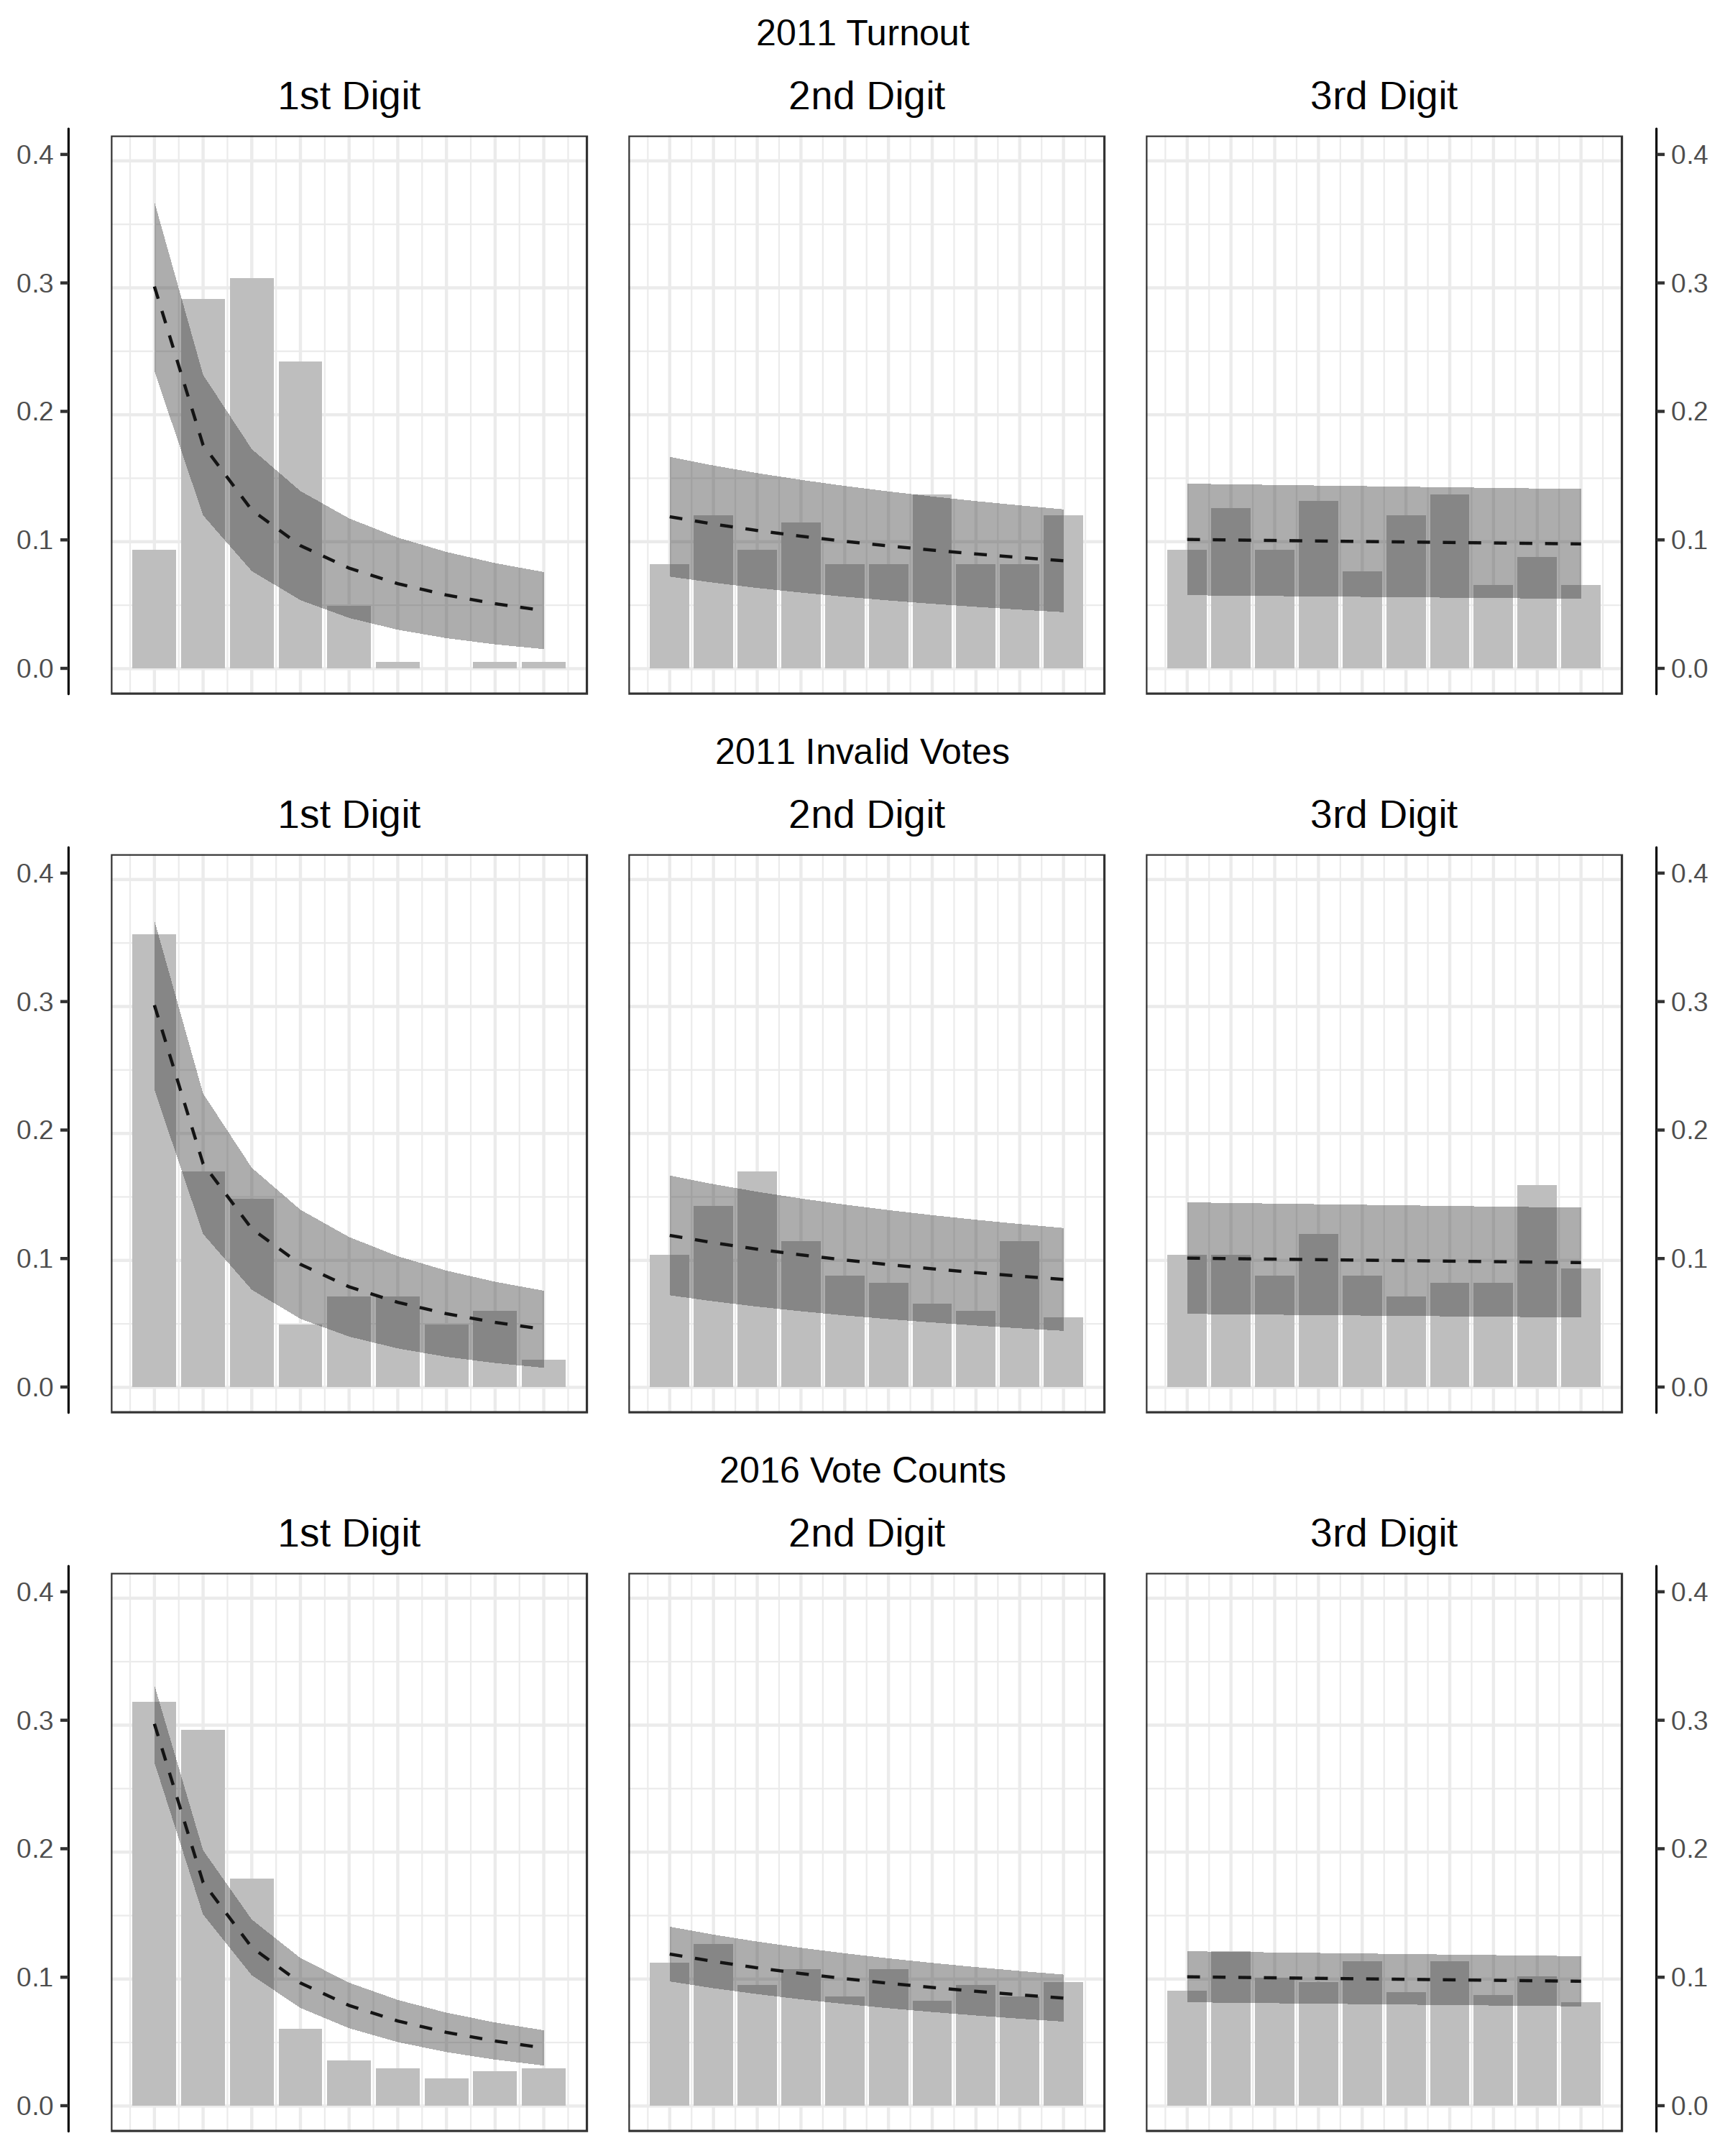
\includegraphics[width=\textwidth]{figure/BENFORD_DIGIT_TEST.png}
	\caption[Digit Test of Election Results]{Empirical distribution (as bars) and expected distribution under Benford's Law (as dashed lines) of first, second, and third digits of district-level voter turnouts in the 2011 election, district-level invalid vote counts in the 2011 election, and district-level vote counts by candidate in the 2016 election. Shaded regions denote 95\% confidence intervals around the expected distributions.}
	\label{fig:Benford}
\end{figure}

\end{document}
